\documentclass[11pt,b5paper]{memoir}

\title{An introduction to computernetworks}
\author{Tom Marcoen}
\date{2022}

\usepackage{xcolor}
\definecolor{spot1}{cmyk}{.67,0  ,.36,0  } % green-blue
\definecolor{spot2}{cmyk}{0  ,.89,.29,0  } % pink
\definecolor{spot3}{cmyk}{1  ,.94,0  ,.50} % dark blue

\colorlet{linkcolor}{spot2}
%%
%% Medtronic color palette
%%

\usepackage{xcolor}

% Primary blue color palette
\definecolor{mdtnavyblue}{cmyk}{1,.94,.47,.43}
\definecolor{mdtmedtronicblue}{cmyk}{.99,.74,.17,.04}
\definecolor{mdtcobaltblue}{cmyk}{.81,.35,0,0}
\definecolor{mdtmediumblue}{cmyk}{.73,.12,0,0}
\definecolor{mdtskyblue}{cmyk}{.55,.04,.04,0}
\definecolor{mdtlightblue}{cmyk}{.29,.05,.05,0}

% Primary neutral color palette
\definecolor{mdtcharcoal}{rgb}{.83,.86,.90}
\definecolor{mdtbluegray}{cmyk}{.68,.40,.28,.08}
\definecolor{mdtdarkgray}{cmyk}{0,0,0,.55}
\definecolor{mdtlightgray}{cmyk}{0,0,0,.30}
\definecolor{mdtpalegray}{cmyk}{.08,.06,.06,0}

% Accent colors
\definecolor{mdtyellow}{cmyk}{0,.18,.93,0}
\definecolor{mdtlightorange}{cmyk}{.02,.38,.96,0}
\definecolor{mdtorange}{cmyk}{.04,.78,1,0}
\definecolor{mdtpurple}{cmyk}{.38,.98,0,0}
\definecolor{mdtgreen}{cmyk}{.57,.02,1,0}
\definecolor{mdtturquoise}{cmyk}{.70,0,.38,0}

\usepackage[utf8]{inputenc}
\usepackage{csquotes}
\usepackage[dutch]{babel}

\usepackage[T1]{fontenc}
\usepackage{libertine}
%\useosf
\usepackage{microtype}

\usepackage{textcomp}
\usepackage[varqu,varl]{inconsolata}
\usepackage{graphicx}
\graphicspath{{images/}}
\setkeys{Gin}{width=.75\textwidth} % from the graphicx package
\setfloatlocations{figure}{hbp}
\setfloatlocations{table}{htp}
\usepackage{caption}
\usepackage{subcaption}
\usepackage{multirow}
\usepackage{siunitx}


\usepackage{contour}
\usepackage{ifthen}
\usepackage{standalone}
% TikZ/PGF
\usepackage{tikz}
\usetikzlibrary{backgrounds}
\usetikzlibrary{calc}
\usetikzlibrary{decorations.pathreplacing}
\usetikzlibrary{fit}
\usetikzlibrary{matrix}
\usetikzlibrary{patterns}
\usetikzlibrary{positioning}
\usetikzlibrary{shapes.geometric}
\usetikzlibrary{arrows}

%%
%% Styles
%%

% Network nodes
\tikzset{network node image/.style={
                inner sep=0mm,
                %anchor=south west
                }}
\tikzset{network node/.style={
                network node image,
                thick,
                text=mdtmedtronicblue,
                draw=mdtmedtronicblue,
                fill=white,
                minimum size=10mm}}
\tikzset{network node circle/.style={
                network node,
                circle}}
\tikzset{network node square/.style={
                network node,
                rectangle,
                rounded corners}}
\tikzset{network node rectangle/.style={
                network node,
                rectangle,
                minimum height=15mm,
                rounded corners}}
\tikzset{server rack/.style={
                align=left,
                text width=8mm,
                inner sep=0pt,
                anchor=north west,
                minimum height=7.5mm-.8pt,
                minimum width=10.7mm-.8pt,
                thick,
                text=mdtmedtronicblue,
                draw=mdtmedtronicblue,
                fill=white}}
\tikzset{network rack/.style={
                align=left,
                text width=9.3mm,
                inner sep=0pt,
                anchor=north west,
                minimum height=7.5mm-.8pt,
                minimum width=12mm-.8pt,
                %minimum height=7.5mm,
                %minimum width=12mm,
                thick,
                text=mdtmedtronicblue,
                draw=mdtmedtronicblue,
                fill=white}}
\tikzset{patch rack/.style={
                align=left,
                text width=9.3mm,
                inner sep=0pt,
                anchor=north west,
                minimum height=7.5mm-.8pt,
                minimum width=12mm-.8pt,
                thick,
                text=mdtmedtronicblue,
                draw=mdtmedtronicblue,
                fill=white}}

% Labels
\tikzset{interface label/.style={
                font=\footnotesize,
                inner sep=2pt},
                fill=white}
\tikzset{node label/.style={
                font=\small,
                align=center,
                inner sep=2pt,
                thick,
                rounded corners}}


% Floor tiles
\newcommand{\dcfloortiles}[2]{%
    \draw[step=6mm,gray,very thin] (0,0) grid ($.6*(#1,#2)$);
}
\newcommand{\dccoldaisle}[2]{%
    \draw[pattern=north west lines, pattern color=mdtlightgray] ($.6*(#1)-(.6,.6)$) rectangle ($.6*(#1)+.6*(#2)-(.6,.6)$);
}
% Markings for different types of racks
\newcommand{\caserack}[1]{%
    \draw[very thick,mdtorange] ($(#1.north east)-(.1,.1)$) -- ($(#1.south east)+(-.1,.1)$);
}
\newcommand{\storagerack}[1]{%
    \draw[very thick,mdtgreen] ($(#1.north east)-(.2,.1)$) -- ($(#1.south east)+(-.2,.1)$);
}
\newcommand{\networkrack}[1]{%
    \draw[very thick,mdtmediumblue] ($(#1.north east)-(.15,.1)$) -- ($(#1.south east)+(-.15,.1)$);
}
\newcommand{\mitgrack}[1]{%
    \draw[very thick,mdtpurple] ($(#1.north east)-(.25,.1)$) -- ($(#1.south east)+(-.25,.1)$);
}
\newcommand{\unixrack}[1]{%
    \draw[very thick,mdtdarkgray] ($(#1.north east)-(.3,.1)$) -- ($(#1.south east)+(-.3,.1)$);
}
\newcommand{\computerack}[1]{%
    \draw[very thick,mdtturquoise] ($(#1.north east)-(.35,.1)$) -- ($(#1.south east)+(-.35,.1)$);
}
\newcommand{\racklabels}[1]{%
    \matrix (racklabels) at (#1) [matrix of nodes,
        nodes={
            anchor=west,
            align=left
            }
        ] {
            |[mdtorange]| CASE \\
            |[mdtturquoise]| Compute (CORE) \\
            |[mdtpurple]| MITG \\
            |[mdtmediumblue]| Network \\
            |[mdtgreen]| Storage \\
            |[mdtdarkgray]| UNIX \\
    };
}
%
% layers.tex
%
% This document contains code to hide a PGF layer if so desired,
% e.g. you can hide the layer with all the labels on it.
%

% Define the layers to be used
\pgfdeclarelayer{connections}
\pgfdeclarelayer{interfaces}
\pgfdeclarelayer{hostnames}
\pgfdeclarelayer{labels}
\pgfdeclarelayer{arrows}

% Make the background white so we can hide the labels by swapping the order of the layers
\tikzset{show background rectangle,background rectangle/.style={rounded corners,fill=white}}

% \showalllayers - Show the nodes, connections, and detailed labels, including interface labels
% The left most layer is the bottom layer; everything left from the background will be hidden.
\newcommand\showalllayers{      \pgfsetlayers{hostnames,arrows,background,connections,main,interfaces,labels}}
\newcommand\showarrows{         \pgfsetlayers{hostnames,background,connections,main,interfaces,labels,arrows}}
% \hidelabels - Show only the nodes and the connections
\newcommand\hidelabels{         \pgfsetlayers{hostnames,arrows,interfaces,labels,background,connections,main}}
% \hideinterfaces - Hide only the interface labels
\newcommand\hideinterfaces{     \pgfsetlayers{hostnames,arrows,interfaces,background,connections,main,labels}}
% \showonlyhostnames - Hide everything but show the hostnames only
\newcommand\showonlyhostnames{  \pgfsetlayers{arrows,interfaces,labels,background,connections,main,hostnames}}
\newcommand\showhostnamesinterfaces{ \pgfsetlayers{arrows,labels,background,connections,main,hostnames,interfaces}}
% Default setting is to show all layers
\showalllayers
%
% connections.tex
%
% This document contains all the commands needed to create connections between
% different network nodes, e.g.
%  - a normal connection, with our without labels.
%  - a vPC connection between 3 or 4 nodes.
%

%
% Syntax:
% \connect[<color>]{<node1>}{<intf1>}{<node2>}{<intf2>}
\newcommand{\connect}[5][black]{

    % Save the coordinates for the interface labels
    \path (#2) -- (#4) coordinate[very near start] (i1) coordinate[midway] (im) coordinate[very near end] (i2);
    
    % Draw the connection between the two devices on the correct layer.
    \begin{pgfonlayer}{connections}
      \draw[color=#1] (#2) -- (#4);
    \end{pgfonlayer}
    
    % Draw the interface labels on the correct layer.
    \begin{pgfonlayer}{interfaces}
        \ifthenelse{\equal{#3}{}}{}{\node[interface label,fill=white] at (i1) {\contour{white}{#3}};}
        \ifthenelse{\equal{#5}{}}{}{\node[interface label,fill=white] at (i2) {\contour{white}{#5}};}
    \end{pgfonlayer}
    
    %\ifthenelse{\equal{#5}{}}{
    %    % Parameter 5 is empty:
    %    \ifthenelse{\equal{#3}{}}{
    %        % Parameter 3 is empty: no interfaces have been given.
    %        \draw[color=#1] (#2) -- (#4);
    %    }{
    %        % Both devices share the same interface name.
    %        \draw[color=#1] (#2) -- (#4)
    %            node [midway,interface] {#3};
    %    }
    %}{
    %    % Parameter 5 is not empty: both interfaces are given.
    %    \draw[color=#1] (#2) -- (#4)
    %        node [on background layer,near start,interface] {#3}
    %        node [near end,interface] {#5};
    %}
}

%
% Syntax:
% \connectClusters[<straight/cross>]{cluster1}{cluster2}
\newcommand{\connectClusters}[3][S]{
    \message{connectClusters 2-1: #2-1^^J}
    \message{connectClusters 2-2: #2-2^^J}
    \message{connectClusters 3-1: #3-1^^J}
    \message{connectClusters 3-2: #3-2^^J}
    \ifthenelse{\equal{#1}{S}}{
        \connect{#2-1}{}{#3-1}{}
        \connect{#2-2}{}{#3-2}{}
    }{
        \connect{#2-1}{}{#3-2}{}
        \connect{#2-2}{}{#3-1}{}
    }
}

%
% Syntax:
% \arrowcoords[<position>]{<coordinates start>}{<coordinates end>}{<text>}
\newcommand{\arrowcoords}[4][midway]{
    \draw[mdtgreen, arrows={-latex'}, shorten <= 0.25cm, shorten >= 0.25cm, very thick, distance=2cm] (#2) to[out=230,in=170] (#3) node[#1] {#4};
}

%
%
%

\def\iconset{3015}


%
% Display only the icons
%
% Syntax: \icon<type>{<hostname>}{<coordinates>}
%

\newcommand{\iconcloud}[2]{
    \node[network node image] (#1) at (#2) {
\includegraphics[width=30mm]{images//cloud.png}};
    \node at ([yshift=-2mm]#2) {#1};
}
\newcommand{\iconfirewall}[2]{
    \ifthenelse{\equal{\iconset}{basic}}{
        \node[network node circle,draw=mdtorange] (#1) at (#2) {FW};
    }{
        \node[network node image] (#1) at (#2) {
\includegraphics[width=10mm]{images/\iconset/firewall.eps}};
    }
}
\newcommand{\iconips}[2]{
    \ifthenelse{\equal{\iconset}{basic}}{
        \node[network node square] (#1) at (#2) {IPS};
    }{
        \node[network node image] (#1) at (#2) {\includegraphics[width=10mm]{images/\iconset/ips.eps}};
    }
}
\newcommand{\iconrouter}[2]{
    \ifthenelse{\equal{\iconset}{basic}}{
        \node[network node circle] (#1) at (#2) {RTR};
    }{
        \node[network node image] (#1) at (#2) {
\includegraphics[width=10mm]{images/\iconset/router.eps}};
    }
    \message{iconrouter: #1^^J}
}
\newcommand{\iconswitch}[2]{
    \ifthenelse{\equal{\iconset}{basic}}{
        \node[network node square] (#1) at (#2) {SW};
    }{
        \node[network node image] (#1) at (#2) {
\includegraphics[width=13mm]{images/\iconset/switch.eps}};
    }
}
\newcommand{\icondistswitch}[2]{
    \ifthenelse{\equal{\iconset}{basic}}{
        \node[network node square] (#1) at (#2) {SW};
    }{
        \node[network node image] (#1) at (#2) {\includegraphics[width=13mm]{images/\iconset/l3switch.eps}};
    }
}
\newcommand{\iconcoreswitch}[2]{
    \ifthenelse{\equal{\iconset}{basic}}{
        \node[network node square] (#1) at (#2) {SW};
    }{
        \node[network node image] (#1) at (#2) {\includegraphics[width=13mm]{images/\iconset/coreswitch.eps}};
    }
}
\newcommand{\iconhost}[2]{
   \ifthenelse{\equal{\iconset}{basic}}{
      \node[network node square] (#1) at (#2) {PC};
   }{
      \node[network node square] (#1) at (#2) {PC};
   }
}



%
% Display the node: icon + labels
%
%
% Syntax: \node<type>[<label position>]{<name>}{<coordinates>}{<type>}{<IP address>}
%
% Where:
%  - <label position> : top, bottom, left, right (default)
%  - <type> : hardware type, e.g. Catalyst 3850
%

\newcommand{\nodecloud}[5][right]{
    \iconcloud{#2}{#3}
}
\newcommand{\nodefirewall}[5][right]{
    \iconfirewall{#2}{#3}
    \nodelabel[#1]{#3}{#2}{#4}{#5}
}
\newcommand{\nodeips}[5][right]{
    \iconips{#2}{#3}
    \nodelabel[#1]{#3}{#2}{#4}{#5}
}
\newcommand{\noderouter}[5][right]{
    \iconrouter{#2}{#3}
    \nodelabel[#1]{#3}{#2}{#4}{#5}
}
\newcommand{\nodedistswitch}[5][right]{
    \icondistswitch{#2}{#3}
    \nodelabel[#1]{#3}{#2}{#4}{#5}
}
\newcommand{\nodeswitch}[5][right]{    
    \iconswitch{#2}{#3}
    \nodelabel[#1]{#3}{#2}{#4}{#5}
}
\newcommand{\nodecoreswitch}[5][right]{    
    \iconcoreswitch{#2}{#3}
    \nodelabel[#1]{$(#3)-(0,.4)$}{#2}{#4}{#5}
}
\newcommand{\nodehost}[5][right]{
   \iconhost{#2}{#3}
   \nodelabel[#1]{#3}{#2}{#4}{#5}
}



%
% Clusters of nodes
%
% Syntax: \cluster<type>[<label position>]{<name>}{<coordinates>}{<type>}{<IP address>}
%

\newcommand{\clustercloud}[3][bottom]{
    \draw[network node,draw=mdtpurple,fill=mdtpalegray] (#3) ellipse (15mm and 10mm);
    \node (#2) at (#3) {#2};
    \ifthenelse{\equal{#1}{top}}{
        \coordinate (a) at ($(#3)-(10mm,-7mm)$);
        \coordinate (b) at ($(#3)+(10mm,7mm)$);
    }{
        \coordinate (a) at ($(#3)-(10mm,7mm)$);
        \coordinate (b) at ($(#3)+(10mm,-7mm)$);
    }
    \message{clustercloud: #2-1^^J}
    \iconrouter{#2-1}{a}
    \message{clustercloud: #2-2^^J}
    \iconrouter{#2-2}{b}
}

\newcommand{\clusterfirewall}[5][bottom]{
    \coordinate (left) at ($(#3)-(1,0)$);
    \coordinate (right) at ($(#3)+(1,0)$);
    \iconfirewall{#2-1}{left}
    \iconfirewall{#2-2}{right}
    
    \begin{pgfonlayer}{connections}
        \node (#2) [draw=mdtmedtronicblue,rounded corners,inner sep=2mm,dashed,fit=(#2-1) (#2-2)] {};
    \end{pgfonlayer}
    \connect{#2-1}{}{#2-2}{}
    
    \nodelabel[#1]{#3}{#2}{#4}{#5}
}




%
% Syntax:
% \nodelabel[<position>]{<coordinates>}{<hostname>}{<type>}{<IP address>}
\newcommand{\nodelabel}[5][right]{
    \def\text{\contour{white}{\textbf{#3}}\\\contour{white}{\emph{#4}}\\\contour{white}{#5}}
    \begin{pgfonlayer}{labels}
    
    % On the right
    \ifthenelse{\equal{#1}{right}}{
        %\node[node label,anchor=west] at ($(#2)+(1,0)$) {\contour{white}{\textbf{#3}\\\emph{#4}\\#5}};
        \node[node label,anchor=west] at ($(#2)+(1,0)$) {\text};
        
    % On the left
    }{\ifthenelse{\equal{#1}{left}}{
        \node[node label,anchor=east] at ($(#2)-(1,0)$) {\text};
    
    % At the top
    }{\ifthenelse{\equal{#1}{top}}{
        \node[node label,anchor=south] at ($(#2)+(0,1)$) {\text};
    
    % At the bottom
    }{\ifthenelse{\equal{#1}{bottom}}{
        \node[node label,anchor=north] at ($(#2)-(0,1)$) {\text};
    
    }{}}}}
    
    \end{pgfonlayer}
    
    \begin{pgfonlayer}{hostnames}
        \node[node label,anchor=north] at ($(#2)-(0,.6)$) {\contour{white}{#3}};
    \end{pgfonlayer}
}

%
% Syntax:
% \vlaninformationR[<xshift>]{<node name>}{<relative location>}
%\newcommand{\vlaninformationR}[4][5cm]{
%    \matrix (#2) [matrix of nodes,
%        right=of #3,
%        xshift=#1,
%        left delimiter=\{,
%        nodes={
%            anchor=west,
%            align=left
%            }
%        ] {
%            #4
%    };
%}
\usepackage{pgf-pie}


\usepackage{varioref}
\usepackage{hyperref}
\usepackage[noabbrev]{cleveref}
\urlstyle{rm}
\hypersetup{colorlinks=true,allcolors=linkcolor,linktocpage}
%\usepackage{geometry}
%\geometry{a4paper,top=30mm,bottom=65mm,left=30mm,right=65mm,footskip=30mm}
%\settypeblocksize{555pt}{*}{.617}
% s = w/8
%\setlrmargins{26.25mm}{*}{*}
%\setheadfoot{\baselineskip}{3\baselineskip}
%\setheaderspaces{*}{\baselineskip}{*}
%\setmarginnotes{2\baselineskip}{45mm}{.6\baselineskip}
%\checkandfixthelayout
\raggedbottom

\pagestyle{ruled}
\frenchspacing



% lists
\RequirePackage{enumitem}
\newlist{inlinelist}{enumerate*}{1}
\setlist*[inlinelist,1]{%
  label=(\roman*),
}
\firmlists
\renewcommand*{\descriptionlabel}[1]{\hspace\labelsep\scshape #1 --}

% Side notes
\strictpagechecktrue
\newcommand{\sidenote}[1]{%
    \checkoddpage%
    \ifoddpage%
    \marginpar{\begin{flushleft}\footnotesize#1\end{flushleft}}%
    \else%
    \marginpar{\begin{flushright}\footnotesize#1\end{flushright}}%
    \fi%
}

% Figures and tables
\usepackage{caption}
\DeclareCaptionLabelFormat{bringhurst}{\scshape\textls[50]{\MakeLowercase{#1}\,#2}}
\captionsetup{font={sf,small},labelformat=bringhurst,format=hang}



\newcommand*{\abbr}[1]{%
   % Format abbreviations as small capitals
   \texorpdfstring{\textsc{\MakeLowercase{#1}}}{#1}%
}
\newcommand{\hostname}[1]{\texttt{#1}}

\usepackage[backend=biber]{biblatex}
\addbibresource{frankenstein/resources.bib}
%\usepackage{glossaries}
%\makeglossaries


\begin{document}
% ====================================
% COVER PAGE
% ====================================

% ====================================
% HALF-TITLE PAGE
% ====================================
%\clearforchapter
%\vspace*{3cm}
%\begin{center}
%   \large{\textsc{\MakeLowercase{\thetitle}}}
%\end{center}
%\thispagestyle{empty}

% ====================================
% TITLE PAGE
% ====================================
%\clearforchapter
%\maketitle
%\thispagestyle{empty}

\pagenumbering{Alpha}
\makeatletter
\begin{titlingpage} % Suppresses displaying the page number on the title page and the subsequent page counts as page 1
\thispagestyle{empty}
	\raggedleft % Right align the title page
	
	\rule{1pt}{\textheight} % Vertical line
	\hspace{0.05\textwidth} % Whitespace between the vertical line and title page text
	\parbox[b]{0.75\textwidth}{ % Paragraph box for holding the title page text, adjust the width to move the title page left or right on the page
		
		{\Huge\bfseries\@title}\\[2\baselineskip] % Title
		{\large\textit{\subtitle}}\\[4\baselineskip] % Subtitle or further description
		{\Large\SC{\@author}} % Author name, lower case for consistent small caps
		
		\vspace{0.5\textheight} % Whitespace between the title block and the publisher
		
		{\noindent 
\includegraphics[width=6cm]{images/logo-cropped.pdf}}\\[\baselineskip] % Publisher and logo
	}

\end{titlingpage}
\makeatother
\frontmatter
\chapter{Preface}

This manual was written as a summary and companion guide to the course titled ``Computernetwerken met \abbr{TCP}/\abbr{IP}''\footnote{This title translates to \emph{Computer networks with} \abbr{TCP}/\abbr{IP}.} that I teach at Syntra Bizz.
Although I teach that course in Dutch, this companion is written in English and this for two reasons.
First of all this allows me to reach a wider audience with this manual.
Secondly, it is difficult to write a technology book in Dutch, given that so many terms are in English.
I found it too difficult to decide which technical terms to translate from English to Dutch.
It is impossible to translate every technical term and translating none of them -- which is really the best option so that it would be easier to search for the terms online to find more resources on them -- would make the text a real mix of Dutch and English.
I decided it is better to write the complete text in English.

I teach the accompanying course in three days of six hours each for a total of eightteen hours of in-class training.
Additionally I expect the students to make lab exercises at home.
Should you consider doing these labs in class also, the course would take about a forty-hour work week.
The schedule for the course is given in \vref{tab:course-schedule}.

\begin{table}
   \centering
   \begin{tabular}{rlll}
                       & \textit{day 1} & \textit{day 2}       & \textit{day 3}   \\[1ex]
   \textit{morning}    & \abbr{IP} addressing  & \abbr{TCP}/\abbr{UDP} and Ethernet & cabling en Wi-Fi  \\
   \textit{afternoon}  & Packet Tracer  & \abbr{VLAN} and \abbr{STP}       & applications     \\
   \end{tabular}
   \caption{In-class course schedule}
   \label{tab:course-schedule}
\end{table}

This manual consists of two parts.
The first part covers the topics that I teach in class.
The second part contains examples and exercises.
I assume the students -- and thus also the reader -- have access to Cisco Packet Tracer but really any virtualisation or simulation software will do.
Other possible candidates include \href{https://www.eve-ng.net/}{eve-ng} and \href{https://www.gns3.com/}{GNS3}.

Most of the examples given are using the Cisco IOS syntax but there are also examples for Juniper Networks' Junos.
Example configuration snippets for other products, such as HP ProCurve or the newer Aruba switches might be added in the future.
%, Aruba's ArubaOS and HP ProCurve.

Last but not least, I welcome constructive feedback at info@marcoen.net.
\tableofcontents
\chapter{Introduction}

A computer network is a set of computers sharing resources.
These computers, as well as the network devices interconnecting them, are also called \emph{network nodes}.
The interconnections between these nodes are either made up of physical cables or by using wireless radio frequencies.
Examples of these interconnections include fiber optic cabling, twisted pair, coax, Wi-Fi, Bluetooth, and \abbr{5G}.



\section{The size of a network}

We can categories computer network depending on their geographical size.
A small network spanning a local area, e.g.~a house or office building, is called a \emph{local area network} or \abbr{LAN}.
A large network spanning a country, continent or even the entire world, is called a \emph{wide area network} or \abbr{WAN}.
The networks operated by Internet service providers are such examples but the best known example is of course the Internet itself.

There are several categories in between these two extremes, for example a campus area network (\abbr{CAN}) or metropolitan area network (\abbr{MAN}) but these terms are not that widely used.
The term \abbr{SAN} or \emph{storage area network} is in common use, however, and refers to a network connecting storage appliances together.



\section{Network topologies}

Apart from their physical size we can also categorise networks based on their topology.
There is a difference between the physical topology -- how the cables go -- and the logical topology -- how the data flows through the network.
Let's start off with the most simple topology: a point-to-point link between two devices.
Examples include a serial cable connecting a terminal to the computer, a direct connection using a \abbr{UTP} cable, or an infrared connection.

Next consider the ring topology in \vref{fig:intro-topo-ring}.
Note that this can be considered a series of point-to-point links.
There is a big difference between a ring topology and a series of point-to-point links, however.
Where a series of point-to-point links can still function correctly when one of the links is broken, a ring topology requires the ring to be intact.
This is because the ring topology uses a protocol that passes a token around the ring used for deciding when a host can put data on the ring.
Examples of a ring topology include \abbr{FDDI} and Token Ring, both of which no longer exist.


\begin{figure}
   \centering
   Ring topology
   \caption{Computers connected in a ring topology}
   \label{fig:intro-topo-ring}
\end{figure}


This ring topology can be both a physical and a logical ring, or it could be a physical star topology and a logical ring topology.
An example is Token Ring which has a central \emph{media access unit} (\abbr{MAU}) to which all computers connect.
The \abbr{MAU} makes sure all devices are logically connected in a ring and, when a cable gets disconnected or a device is turned off, the \abbr{MAU} skips that link and restores the ring with the remaining devices.

Both Thicknet and Thinnet form a physical and logical bus topology (\vref{fig:intro-topo-bus}) with all devices connecting to a long cable.
Ethernet hubs form a physical star topology with the hub being the centre, much like the \abbr{MAU} in a Token Ring network.
Logically the Ethernet network operates just like the Thinnet bus topology as all devices receive all traffic on the wire.
An Ethernet switch changes this behavior as it isolates the differnet cable segments from each other.
It thus forms both a physical and a logical star topology.


\begin{figure}
   \centering
   Bus topology
   \caption{Computers connected in a bus topology}
   \label{fig:intro-topo-bus}
\end{figure}

A mesh topology interconnects all devices with each other.
A \emph{full mesh} (\vref{fig:intro-topo-full-mesh}) connects every device with every other device while in a \emph{partial mesh} (\vref{fig:intro-topo-partial-mesh}) some of the connections are missing.


\begin{figure}
   \begin{subfigure}[b]{.47\textwidth}
      \centering
      FULL MESH
      \caption{A full mesh}
      \label{fig:intro-topo-full-mesh}
   \end{subfigure}
   \hfill
   \begin{subfigure}[b]{.47\textwidth}
      \centering
      PARTIAL MESH
      \caption{A partial mesh}
      \label{fig:intro-topo-partial-mesh}
   \end{subfigure}
   \caption{Meshed networks}
   \label{fig:intro-topo-mesh}
\end{figure}


%Thick- en thinnet gebruiken beide een fysieke busstructuur waarbij alle computers op één lange kabel geprikt worden.
%Beide standaarden gebruiken coax (echter van een andere dikte, vandaar de namen) maar beide gebruiken een andere manier om de computers met het netwerk te verbinden.
%Thicknet gebruikt ``vampire taps'' en een \emph{drop cable} terwijl thinnet BNC-koppelstukken gebruikt.%
%   \footnote{Er was ook een N-connector beschikbaar voor Thicknet maar deze werd blijkbaar amper gebruikt (\href{http://www.mattmillman.com/projects/10base5/}{bron}).}



\section{Network protocols}

A communication protocol is a system of rules that allows two or more entities of a communications system to transmit information.
The protocol defines the rules, syntax, semantics and synchronization of communication and possible error recovery methods.
Protocols may be implemented by hardware, software, or a combination of both.

Multiple protocols often describe different aspects of a single communication.
A group of protocols designed to work together is known as a \emph{protocol suite}; when implemented in software they are a \emph{protocol stack}.

Some of the protocols we will (briefly) cover in this course are \abbr{IP} versions~4 and~6, \abbr{TCP}, \abbr{UDP}, Ethernet, and \abbr{ARP}.
Some of the network protocols which are no longer in use, include \abbr{IPX} and AppleTalk.



\section{A brief history of computer networks}

The first \emph{mainframes} appeared in the fifties.
Data had to be entered using punched cards or mangetic tape.
Output had to be printed as there were no monitors yet.
You first had to load the program into memory and then the date you wished to process.
There were no operating systems yet.
It wasn't until the early seventies when terminals were being used.

\begin{itemize}
\item
   In the late 1950s, a network of computers was built for the U.S. military semi-automatic ground environment (\abbr{SAGE}) radar system using the Bell 101 modem.
   It was the first commercial modem for computers, released by AT\&T Corporation in 1958.
   The modem allowed digital data to be transmitted over regular unconditioned telephone lines at a speed of 110 bits per second~(bit/s).
\item
   In 1959, Christopher Strachey filed a patent application for time-sharing and John McCarthy initiated the first project to implement time-sharing of user programs at MIT.
   Stratchey passed the concept on to J. C. R. Licklider at the inaugural \abbr{UNESCO} Information Processing Conference in Paris that year.
   McCarthy was instrumental in the creation of three of the earliest time-sharing systems (Compatible time-sharing system in 1961, BBN time-sharing system in 1962, and Dartmouth time sharing system in 1963).
\item
   In 1959, Anatoly Kitov proposed to the Central Committee of the Communist Party of the Soviet Union a detailed plan for the re-organisation of the control of the Soviet armed forces and of the Soviet economy on the basis of a network of computing centres.
   Kitov's proposal was rejected, as later was the 1962 OGAS economy management network project.
\item
   In 1960, the commercial airline reservation system semi-automatic business research environment (\abbr{SABRE}) went online with two connected mainframes.
\item
   In 1963, J. C. R. Licklider sent a memorandum to office colleagues discussing the concept of the ``Intergalactic Computer Network,'' a computer network intended to allow general communications among computer users.
\item
   Throughout the 1960s, Paul Baran and Donald Davies independently developed the concept of packet switching to transfer information between computers over a network.
   Davies pioneered the implementation of the concept.
   The \abbr{NPL} network, a local area network at the National Physical Laboratory (United Kingdom) used a line speed of 768 kbit/s and later high-speed T1 links (1.544 Mbit/s line rate).
\item
   In 1965, Western Electric introduced the first widely used telephone switch that implemented computer control in the switching fabric.
\item
   In 1969, the first four nodes of the \abbr{ARPANET} were connected using 50 kbit/s circuits between the University of California at Los Angeles, the Stanford Research Institute, the University of California at Santa Barbara, and the University of Utah.
   In the early 1970s, Leonard Kleinrock carried out mathematical work to model the performance of packet-switched networks, which underpinned the development of the \abbr{ARPANET}.
   His theoretical work on hierarchical routing in the late 1970s with student Farouk Kamoun remains critical to the operation of the Internet today.
\item
   In 1972, commercial services were first deployed on public data networks in Europe, which began using X.25 in the late 1970s and spread across the globe.
   The underlying infrastructure was used for expanding \abbr{TCP}/\abbr{IP} networks in the 1980s.
\item
   In 1973, the French \abbr{CYCLADES} network was the first to make the hosts responsible for the reliable delivery of data, rather than this being a centralized service of the network itself.
\item
   In 1973, Robert Metcalfe wrote a formal memo at Xerox \abbr{PARC} describing Ethernet, a networking system that was based on the Aloha network, developed in the 1960s by Norman Abramson and colleagues at the University of Hawaii.
   In July 1976, Robert Metcalfe and David Boggs published their paper ``Ethernet: distributed packet switching for local computer networks'' and collaborated on several patents received in 1977 and 1978.
\item
   In 1974, Vint Cerf, Yogen Dalal, and Carl Sunshine published the Transmission Control Protocol (\abbr{TCP}) specification, \abbr{RFC} 675, coining the term Internet as a shorthand for internetworking.
\item
   In 1976, John Murphy of Datapoint Corporation created \abbr{ARCNET}, a token-passing network first used to share storage devices.
\item
   In 1977, the first long-distance fiber network was deployed by \abbr{GTE} in Long Beach, California.
\item
   In 1977, Xerox Network Systems (\abbr{XNS}) was developed by Robert Metcalfe and Yogen Dalal at Xerox.
\item
   In 1979, Robert Metcalfe pursued making Ethernet an open standard.
\item
   In 1980, Ethernet was upgraded from the original 2.94 Mbit/s protocol to the 10~Mbit/s protocol, which was developed by Ron Crane, Bob Garner, Roy Ogus, and Yogen Dalal.
\item
   In 1995, the transmission speed capacity for Ethernet increased from 10~Mbit/s to 100~Mbit/s.
   By 1998, Ethernet supported transmission speeds of 1~Gbit/s.
   Subsequently, higher speeds of up to 400 Gbit/s were added (as of 2018).
   The scaling of Ethernet has been a contributing factor to its continued use.
\end{itemize}



\section{The \abbr{OSI} and \abbr{TCP}/\abbr{IP} models}

The Open Systems Interconnection (\abbr{OSI}) model is a conceptual model that was developed in the late 1970's for the field of computer networking, and then became an operating model in the 1980's through the International Organization for Standardization (\abbr{ISO}).


Het OSI-model is een conceptueel model voor netwerkcommunicatie.
Het werd als theoretisch model ontwikkeld met de bedoeling dat de praktijk zich aan dit model aan zou passen.
Het TCP/IP-model is een alternatief protocol dat gebaseerd is op de protocollen die al in de praktijk gebruikt werden.

\begin{table}[htp]
   \centering
   \begin{tabular}{rll}
   %\toprule
              & \textsc{osi-model}           & \textsc{tcp/ip-model} \\[1ex]
   %\midrule
   \textit{7} & application                  & \multirow{3}{*}{\textcolor{spot1}{application}} \\
   \textit{6} & presentation                 & \\
   \textit{5} & session                      & \\[1ex]
   \textit{4} & \textcolor{spot1}{transport} & transport \\[1ex]
   \textit{3} & \textcolor{spot1}{network}   & internet \\[1ex]
   \textit{2} & \textcolor{spot1}{data link} & \multirow{2}{*}{link} \\
   \textit{1} & \textcolor{spot1}{physical}  & \\
   %\bottomrule
   \end{tabular}
   \caption{De zeven lagen van het OSI-model en de vier lagen van het TCP/IP-model.
   De vijf lagen van het hybride model zijn in kleur weergegeven.}
   \label{tab:osi-model}
\end{table}

Deze modellen hebben weinig praktisch nut maar kunnen wel helpen met het gestructureerd opsporen en oplossen van netwerkproblemen.
Afhankelijk van het probleem kan je ofwel op laag~7 (de applicatie) beginnen met troubleshooten, ofwel op laag~1 (de bekabeling), ofwel in het midden op laag~3 (het netwerk).
Onderstaand vind je voor de vijf lagen van het hybride model enkele zaken die onderzocht kunnen worden.

\begin{description}
\item[application]
   Controleer de configuratie van de applicatie zelf.
   Dit is aan de applicatie- of systeembeheerders en niet aan de netwerkbeheerder.
\item[transport]
   Controleer firewallconfiguraties en of de service (applicatie) wel gestart is op de server.
   Je kan met behulp van \cmd{telnet} testen of de applicatie bereikbaar is.
\item[network]
   Verifiëer met behulp van \cmd{ping} en \cmd{traceroute} of de twee computers elkaar kunnen bereiken.
   De output van \cmd{traceroute} geeft een indicatie hoe de pakketjes doorheen het netwerk gaan.
   Dit kan je best in beide richtingen controleren aangezien \emph{asymetrisch} netwerkverkeer mogelijk is en mogelijk voor problemen kan zorgen.
\item[data link]
   Op het lokale netwerk moet je zaken zoals Spanning-tree protocol (STP) en VLAN-configuraties nakijken.
   Zaken zoals DHCP snooping, dynamic ARP inspection (DAI) en port security kan je hier ook nakijken.
\item[physical]
  Controleer bekabeling, connectors, interface errors en, in het geval van wifi, mogelijke storingsbronnen.
\end{description}

De verschillende lagen vinden we ook terug als we de verschillende stappen doorlopen die computers doorlopen om met elkaar te communiceren.




\section{Routing schemes}

There are four different routing schemes, or ways to deliver a packet on the network.
\begin{description}
\item[unicast] Unicast delivers a message to a single specific node using a one-to-one association between a sender and destination: each destination address uniquely identifies a single receiver endpoint.
\item[broadcast] Broadcast delivers a message to all nodes in the network using a one-to-all association; a single datagram (or packet) from one sender is routed to all of the possibly multiple endpoints associated with the broadcast address. The network automatically replicates datagrams as needed to reach all the recipients within the scope of the broadcast, which is generally an entire network subnet.
\item[multicast] Multicast delivers a message to a group of nodes that have expressed interest in receiving the message using a one-to-many-of-many or many-to-many-of-many association; datagrams are routed simultaneously in a single transmission to many recipients. Multicast differs from broadcast in that the destination address designates a subset, not necessarily all, of the accessible nodes.
\item[anycast] Anycast delivers a message to any one out of a group of nodes, typically the one nearest to the source using a one-to-one-of-many as\-so\-ci\-a\-tion where datagrams are routed to any single member of a group of potential receivers that are all identified by the same destination address. The routing algorithm selects the single receiver from the group based on which is the nearest according to some distance or cost measure.
\end{description}
We will not cover multicast or anycast in this course.



\section{Communication between computers}



Nemen we als voorbeeld een computer, de \emph{client}, die een webpagina op wil halen van een andere computer, de \emph{server} (\vref{fig:client-server}).
Het protocol dat hier voor gebruikt wordt, heet hypertext transfer protocol (HTTP).
De client verstuurt een HTTP \emph{request} en de server antwoordt met een HTTP \emph{response}.

De request bevat de volgende data.
\begin{verbatim}
GET /index.html HTTP/1.1
Host: www.example.com
\end{verbatim}

\begin{figure}
   \centering
   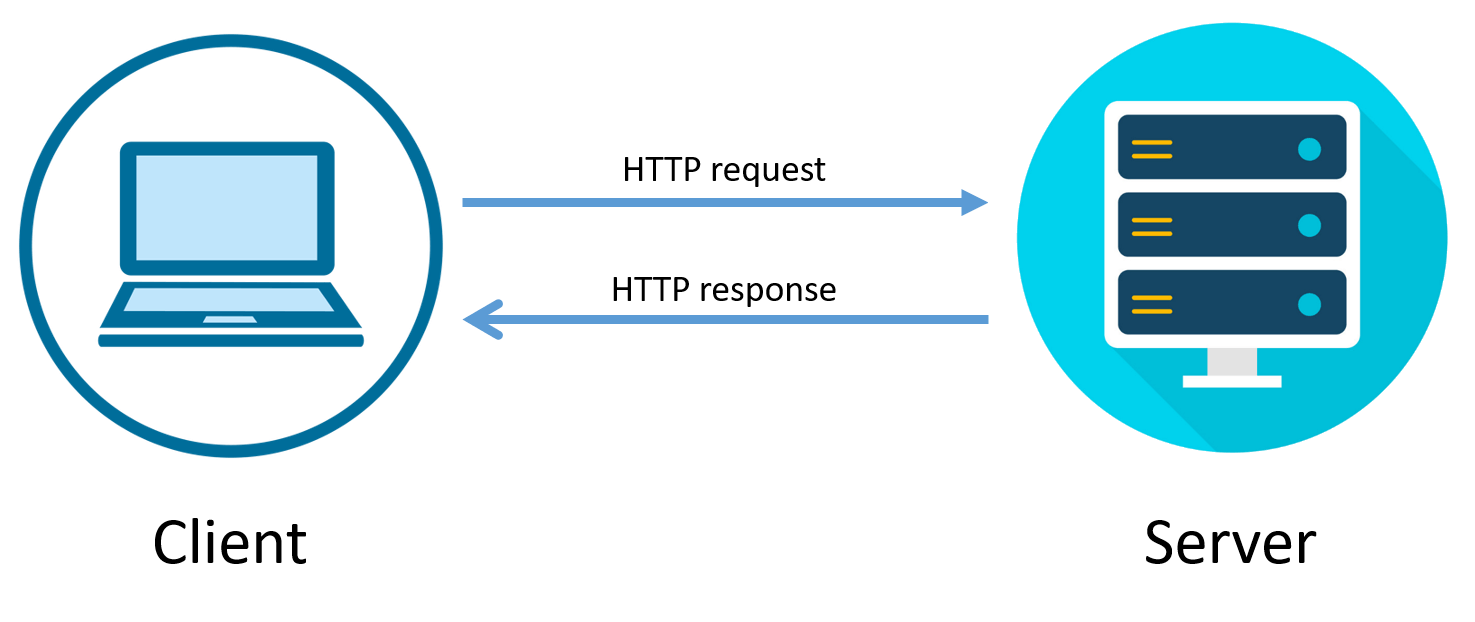
\includegraphics[width=.65\textwidth]{images/http-request.png}
   \caption{Een client vraagt een webpagina op bij eeen webserver en gebruikt voor deze communicatie HTTP}
   \label{fig:client-server}
\end{figure}

Het antwoord van de server bevat enerzijds de HTTP-data die het protocol vereist en anderzijds de gevraagde webpagina.
In dit geval bevat de gevraagde pagina HTML-code.
\begin{verbatim}
HTTP/1.1 200 OK
Content-Type: text/html; charset=UTF-8
Content-Length: 155
Server: Apache/1.3.3.7 (Unix) (Red-Hat/Linux)

<html>
  <head><title>An Example Page</title></head>
  <body><p>Hello World!</p></body>
</html>
\end{verbatim}

Dit ogenschijnlijk eenvoudig voorbeeld roept toch meerdere vragen op.
\begin{enumerate}
\item Hoe kunnen we de server bereiken?
\item Voor welke applicatie is de data bestemd?
\item Hoe versturen we heel veel data?
\item Wat doen we als er iets mis gaat?
\end{enumerate}



\subsection{Hoe kunnen we de server bereiken?}
In de adresbalk van de browser vullen we de \emph{domeinnaam} van de website in die we willen bereiken, bijvoorbeeld \url{www.example.com}.
Deze domeinnaam vinden we ook terug in de Host header van de HTTP request.
Omdat computers met elkaar communiceren door middel van IP-adressen, moet deze domeinnaam eerst omgezet worden in een IP-adres.
Dit gebeurt met behulp van het Domain Name System (DNS).

\subsection{Voor welke applicatie is de data bestemd?}
Als pakketjes aankomen op een server of client computer, moet het besturingssysteem weten voor welke applicatie ze bestemd zijn.
Bevatten de pakketjes een email bestemd voor Outlook of een gif van een kat die in de browser getoond moet worden?
Elk programma dat communiceert op het netwerk krijgt een poortnummer toegewezen.
Deze poortnummers worden meegestuurd in de pakketjes zodat de computers steeds weten voor welke applicatie de pakketjes bestemd zijn.
We leren meer over deze poortnummers als we TCP en UDP bespreken.

\subsection{Hoe versturen we heel veel data?}
Als we een groot document door willen sturen, reist de vraag of we dit document als één geheel kunnen sturen, of moeten opsplitsen in kleine stukjes om vervolgens deze kleine stukjes afzonderlijk te versturen.
We zullen merken dat er technische beperkingen zijn die de maximale grootte van een pakket bepalen op sommige netwerken.
Het is soms dus noodzakelijk om grote bestanden op te splitsen en als kleine stukjes te versturen.

Als we een groot bestand opsplitsen in twintig kleine stukjes en deze afzonderlijk versturen, moet de ontvanger van deze twintig pakketjes er wel in slagen om ze alle twintig terug samen te puzzelen tot één geheel.
De ontvanger moet ook zeker dat dat hij alle stukjes ontvangen heeft.
Het is belangrijk dat hij weet dat de verzender twintig pakketjes verstuurd heeft in plaats van eenentwintig.

Deze vraagt hangt ook samen met de volgende vraag.

\subsection{Wat doen we als er iets mis gaat?}
Pakketjes kunnen verloren gaan of er kunnen ``beschadigingen'' optreden in een pakketje (een ``1'' kan een ``0'' worden of omgekeerd).
Pakketjes kunnen in de verkeerde volgorde aankomen.
Dit zijn uitdagingen die TCP en UDP wel (of bewust niet) oplost.




\section{Encapsulatie en decapsulatie}

We gaan nu terug naar de computer die een HTTP request stuurt naar de web server.
De computer heeft een DNS request uitgestuurd voor de domeinnaam www.example.com en kreeg het IP-adres 192.168.1.102.
De HTTP request wordt nu ``ingepakt'' in een TCP-pakket (\vref{fig:transmit-data}).
Dit ``inpakken'' (\emph{encapsulation}) is niet meer dan wat extra data toe te voegen, ofwel voor ofwel na de andere data.
TCP voegt onder andere de nodige poortnummers toe.


\begin{figure}
   \centering
   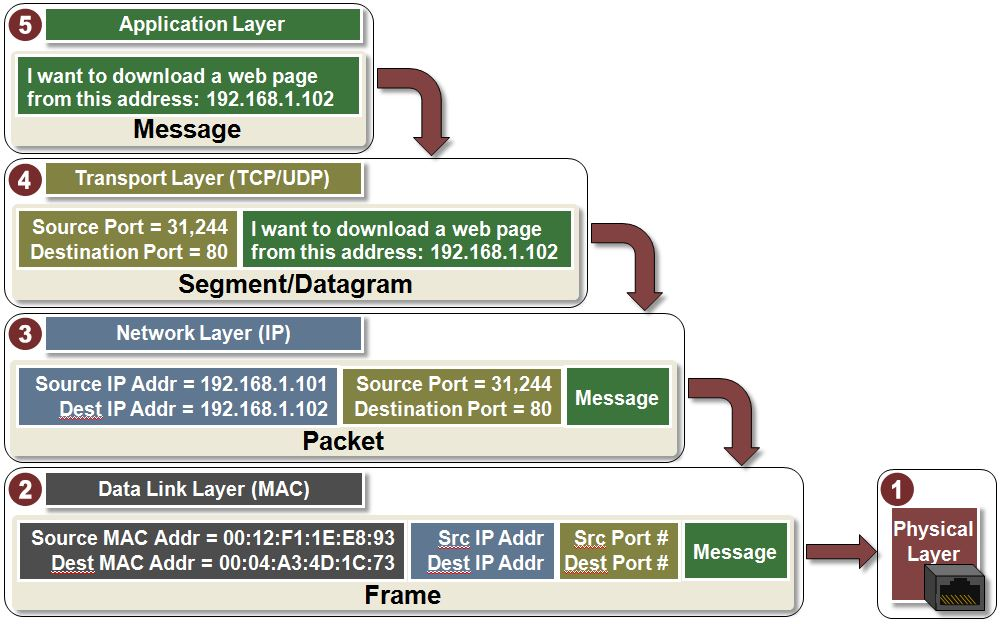
\includegraphics[width=\textwidth]{images/transmit_data.jpg}
   \caption{Elk protocol voegt een eigen header toe aan het pakket}
   \label{fig:transmit-data}
\end{figure}

Vervolgens wordt het pakket doorgegeven aan IP.
Deze voegt de source en destination IP-adressen toe.
Vervolgens voegt Ethernet een header toe met source en destination MAC-adressen waarna het pakket door de netwerkkaart het netwerk wordt opgestuurd.
Dit is de physical layer.


%\begin{frame}{Communicatie gebeurt tussen lagen onderling}
%\begin{center}
%\includegraphics<presentation>[width=\textwidth]{images/tcpip_5_layer_overview.png}
%\includegraphics<article>[width=.65\textwidth]{images/tcpip_5_layer_overview.png}
%\end{center}
%Bron: \url{https://microchipdeveloper.com/}
%\end{frame}
%




\section{Network icons}
\mainmatter
\section{IP-adressen}

\begin{frame}{Netwerken}
\begin{center}
\includegraphics<presentation>[width=.65\textwidth]{images/client-server-2.png}
\includegraphics<article>[width=.65\textwidth]{images/client-server-2.png}
\end{center}
\begin{itemize}
   \item De client en server maken deel uit van een netwerk
   \item Netwerken worden met elkaar verbonden via routers
\end{itemize}
\end{frame}

\mode<article>{
Als we de situatie uit de inleiding in meer detail bekijken, merken we dat zowel de client als de server deel uitmaken van een netwerk en dat deze netwerken met elkaar verbonden worden met behulp van \emph{routers}.
De werking van routers bestuderen we in een later hoofdstuk.
In dit hoofdstuk focussen we op de IP-adressen.
}



\begin{frame}{Netwerkadressen}
\begin{itemize}
\item<1-> Elke computer heeft een IP-adres
    \begin{itemize}
    \item<2-> Mogelijk meerdere IP-adressen
    \end{itemize}
\item<3-> Een IP-adres bestaat uit twee delen:
    \begin{enumerate}
    \item Netwerkdeel
    \item Hostdeel        
    \end{enumerate}
\item<5-> Elk netwerk heeft een eigen, uniek, netwerkdeel
\end{itemize}
\uncover<4>{
   \begin{exampleblock}{Voorbeeld: 192.0.2.1/24}
   \begin{itemize}
   \item Netwerkdeel: 192.0.2
   \item Hostdeel: 1
   \end{itemize}
   \end{exampleblock}
 }
\end{frame}



\begin{frame}{Netwerkadressen: een voorbeeld}
   \begin{center}
      \includegraphics<presentation>[width=.65\textwidth]{images/client-server-3.png}
      \includegraphics<article>[width=.65\textwidth]{images/client-server-3.png}
      \end{center}
\end{frame}



\begin{frame}{IP-adressen}
\begin{itemize}
\item<1->Een IP-adres bestaat uit 32 bits
\item<2->De computer ziet het adres als één getal van 0 tot \num{4294967295}
\item<3->Mensen vinden de \emph{dotted decimal} notatie duidelijker
\item<5->Vier blokjes (\emph{octet}) van 8 bits, gescheiden door een punt
\item<6->Elk octet is een getal van 0 tot 255
\end{itemize}
\uncover<4>{
   \begin{exampleblock}{Voorbeeld}
      \begin{itemize}
      \item 192.0.2.1
      \item 224.0.0.2
      \item 198.15.67.32
      \end{itemize}
      \end{exampleblock}
}
\end{frame}



\begin{frame}{Subnetmasker en prefix-length}
\begin{itemize}
\item<1-> De grootte van het netwerkgedeelte wordt bepaald door de prefix-length
\item<2-> Vanaf links te tellen bepaalt deze het netwerkgedeelte
\item<3-> Deze kan je omzetten naar een subnetmasker
\item<4-> Subnetmaskers zijn de oude manier van noteren
\item<5-> $32-p$ bits vanaf rechts bepalen het hostgedeelte
\end{itemize}
\end{frame}



\begin{frame}{Subnetmaskers}
\begin{exampleblock}{Voorbeelden}
\begin{itemize}
\item<1-> 192.168.23.7/25 \hfill 255.255.255.128 \hspace*{.3\textwidth}\null
\item<2-> 203.0.113.154/26 \hfill 255.255.255.192 \hspace*{.3\textwidth}\null
\item<3-> 172.17.3.22/12 \hfill 255.255.240.0 \hspace*{.3\textwidth}\null
\end{itemize}
\end{exampleblock}
\end{frame}



\begin{frame}{Speciale adressen}
\begin{itemize}
\item Het eerste en laatste adres in een netwerk zijn gereserveerd
\item Het eerste adres is het \alert{netwerkadres}
\item Het laatste adres is het \alert{broadcastadres}
\end{itemize}
\end{frame}


\subsection{Hiërarchische adressen}

\begin{frame}
\end{frame}

\subsection{Variabele groottes van subnetten}

\begin{frame}
\end{frame}



\subsection{Dynamically assigning IP addresses}

\begin{frame}{Static configuration}
\begin{itemize}[<+->]
\item A lot of work
\item Difficult
\item Not only IP address and subnet mask need reconfiguration
\end{itemize}

\only<1>{
   \begin{example}
      Configuring IP settings for thousands of computers in a company
   \end{example}
}
\only<2>{
   \begin{example}
      If you take your laptop to a coffeeshop you do not know their IP settings
   \end{example}
}
\only<3->{
   \begin{example}
      \begin{itemize}[<+->]
      \item DNS settings
      \item TFTP settings (VoIP)
      \end{itemize}
   \end{example}
}
\end{frame}



\begin{frame}{Dynamic Host Configuration Protocol}
\begin{itemize}[<+->]
\item Uses \alert{broadcasts} to exchange packets
\item 
\end{itemize}
\end{frame}

\subsection{Network address translation}

\begin{frame}
\end{frame}
\subsection{IP versie 6}

\begin{frame}
\end{frame}


\chapter{Routing}
\label{chap:routing}

A \emph{router} connects multiple networks together.
\Vref{fig:routing-basic} shows a router in\-ter\-con\-nect\-ing two networks.
When a host of one network wants to communicate with a host on the other network, it can send the traffic to the router.
The router can forward the traffic on to the other network.
Things are easy for this router as there are only two networks and the router knows about both of them as it has an interface in each network.


\begin{figure}
   \centering
   A ROUTER CONNECTING TWO NETWORKS TOGETHER
   \caption{A router connecting two networks together}
   \label{fig:routing-basic}
\end{figure}

Things become a bit more complex in \vref{fig:routing-two-routers}.
Router \hostname{blue} knows about three of the four networks as it has an interface in these three networks.
Router \hostname{red} only knows about two of the four networks.
For \hostname{blue} to be able to send traffic to the fourth network, we must teach \hostname{blue} how to reach this network.
In this case, things are relatively easy: we can tell \hostname{blue} to forward all traffic destined to this fourth network to \hostname{red}, who already knows about this network.
Similarly we need to teach \hostname{red} how to reach the two networks that it does not know about.


\begin{figure}
   \centering
   \caption{Two routers interconnecting a total of four networks}
   \label{fig:routing-two-routers}
\end{figure}


We could manually configure both \hostname{blue} and \hostname{red} but this is repetitive work, error-prone and it does not react well to changes in the network, for example, when a link fails or gets added.
The industry thus developed several protocols for the routers to exchange this information dynamically.
Each router tells its neighbouring routers the networks it knows about.
This way, eventually all routers learn about all networks and they can calculate the best path to reach each network.

In this chapter will first consider static routing in more detail.
Next we will discuss the Routing Information Protocol, a simple yet still widely used protocol for dynamically exchanging network prefixes.
We conclude the chapter with a brief introduction to both Open Shortest Path First and the Border Gateway Protocol.



\section{The router's routing table}

Every host which has an \abbr{IP} address, also has a routing table which tells the device how to forward traffic.
Depending on your operating system you can view the local routing table with \cmd{netstat} or \cmd{route}.
Below is an example for a server running FreeBSD version 13.0-\textsc{release}-p8.
\begin{verbatim}
$ netstat -rnf inet
Routing tables

Internet:
Destination        Gateway            Flags     Netif Expire
default            198.19.208.1       UGS      vtnet0
10.18.0.0/16       link#1             U        vtnet0
10.18.0.5          link#1             UHS         lo0
10.133.0.0/16      link#2             U        vtnet1
10.133.19.35       link#2             UHS         lo0
127.0.0.1          link#3             UH          lo0
198.19.208.0/21    link#1             U        vtnet0
198.19.210.27      link#1             UHS         lo0
\end{verbatim}
I have given three flags to the command.
The first flag (``-r'') tells \cmd{netstat} to list the routing table.
The second flag (``-n'') tells \cmd{netstat} to not resolve hostnames.
Omitting this flag results in ``127.0.0.1'' being shown as ``localhost'' and ``198.19.210.27'' -- which is this host's local IP address -- to be replaced by the hostname of this host.
The third and final option (``-f inet'') makes \cmd{netstat} only display the \abbr{IP} version~4 or \emph{inet4} routing table.

The first column lists the prefix and prefix length with the exception of a \emph{host route} or single \abbr{IP} address, which has a prefix length of 32 bits, and the default route.
The world ``default'' means ``0.0.0.0/0'' or ``no bits have to match,'' i.e.~it accept all possible \abbr{IP} addresses.

The second column lists the \emph{gateway} or router to which to send the packets destined for remote networks.
Only the default route has a gateway listed, which is also sometimes called the \emph{gateway of last resort}.
The other networks are known to the computer as it has an interface in those networks so there is no need for a gateway.

We will skip the flags in the third column.
You can look those up in the documentation.
Finally the last column lists the interface from which to send the packets to their destination.

Now let's take a look at the first two entries -- namely 0.0.0.0/0 and 10.18.0.0/16 -- and assume we want to send a packet destined to 10.18.20.7.
It matches the default route as all packets match this default, but it also matches the first sixteen bits of the 10.18.0.0 prefix.
Which route must it take then?
This brings us to the first important rule about routing tables:

\begin{quote}
   When selecting a route from the routing table, the longest match always wins.
\end{quote}

As the \abbr{IP} address matches the prefix 10.18.0.0/16 with sixteen bits and the prefix 0.0.0.0/0 with zero bits, the packet is sent out on the local network connected to vtnet0.
This happens to be the same interface as the default route is pointed out to but remember the \emph{address resolution protocol} (\abbr{ARP})!
When you send out traffic destined for a directly connected network you send out an \abbr{ARP} request for the destination \abbr{IP} address while when you need to forward the packet to a gateway, you send out an \abbr{ARP} request for that gateway's \abbr{MAC} address (see \vref{sec:arp}).

Before we move on to static routing, let's take a quick look at an example of a routing table on Windows~10.
Note that the command is not \cmd{netstat} but \cmd{route print}.
I have omitted the interface list which is printed at the top as this is not relevant for this example.

\begin{verbatim}
C:\>route print -4
...
Active Routes:
===============================================================
Network Destination        Netmask  Gateway   Interface  Metric
          0.0.0.0          0.0.0.0  10.0.0.1  10.0.0.75      35
         10.0.0.0        255.0.0.0  On-link   10.0.0.75     290
        10.0.0.75  255.255.255.255  On-link   10.0.0.75     290
       10.0.0.255  255.255.255.255  On-link   10.0.0.75     290
        127.0.0.0        255.0.0.0  On-link   127.0.0.1     330
        127.0.0.1  255.255.255.255  On-link   127.0.0.1     330
  127.255.255.255  255.255.255.255  On-link   127.0.0.1     330
        224.0.0.0        240.0.0.0  On-link   127.0.0.1     330
        224.0.0.0        240.0.0.0  On-link   10.0.0.75     290
  255.255.255.255  255.255.255.255  On-link   127.0.0.1     330
  255.255.255.255  255.255.255.255  On-link   10.0.0.75     290
===============================================================
Persistent Routs:
  None
\end{verbatim}




\section{Static routes}
\label{sec:routing-static}

Although I made them sound as something terrible and to-be avoided, static routes are very useful and are still used extensively in companies both small and large.
Somtimes there is only one way out and then it does not make sense to run a routing protocol.

Let's start with the example in \vref{fig:routing-home-network}.
The only way out for your home router is via the ISP router.
A simple static default route will thus suffice.
A \emph{default route} is the name given to the prefix 0.0.0.0/0 meaning that zero bits (due to the prefix length being zero) have to match the given prefix 0.0.0.0.
This matches all possible IP addresses.


\begin{figure}
   \centering
   Cloud -- ISP router -- home router -- local network (switch) with two computers
   \caption{A home router connecting your local network to the Internet}
   \label{fig:routing-home-network}
\end{figure}


\Vref{fig:routing-static-vpn} shows a second example for static routing.
Two offices are connected to the Internet and have an IPsec \abbr{VPN} tunnel configured between them.
For the devices in the first office to reach the devices in the other office through the tunnel, you can configure a static routing directing the network traffic for the other network through the tunnel interface.


\begin{figure}
   \centering
   Two networks connecting to the Internet and a \abbr{VPN} tunnel between them
   \caption{Static routing is often used to direct traffic through a \abbr{VPN} tunnel}
   \label{fig:routing-static-vpn}
\end{figure}


The third example is one from the big enterprises and service providers.
They tend to have a separate management network (\vref{fig:routing-static-management}).
Servers have their default gateway pointing out the public interface but need to send all management traffic out their secondary interface designated for management.


\begin{figure}
   \centering
   Server connecting to a ``public'' network and a management network
   \caption{Large enterprises and service providers tend to have separate management networks requiring static routing to be configured on the servers}
   \label{fig:routing-static-management}
\end{figure}



\section{Dynamic routing protocols}
\label{sec:routing-dynamic}

In specific simple network topologies static routing is perfectly suitable to provide connectivity between routers.
However, most networks are not this simplistic and a dynamic routing protocol then makes life a lot easier.

There are two kinds of dynamic routing protocols: \emph{distance-vector} and \emph{link-state} protocols.
A distance-vector routing protocol calculates the best routes to reach every network that it knows and then sends this information to its neighbours as a vector containing distance and direction.
You can compare these vectors to the fingerposts you see on crossroads.
They list the cities you can reach, the direction to go to and the distance you have to travel before reaching your destination.
A router using a distance-vector routing protocol does not know the detailed information on the different paths available.
It only knows that the best (shortest) route is a given direction.
This is also sometimes called \emph{routing by rumour}.

Link-state routing protocols are comparable to a street map.
Every router sends updates throughout the network indicating which networks it is connected to.
A router can use the updates from all other routers to construct a complete network map.
It knows exactly which router connects to which and where each network is located.
It will then calcuate the best route based on this information.

The Routing Information Protocol (\abbr{RIP}) and the Enhanced Interior Gateway Routing Protocol (\abbr{EIGRP}) are both examples of distance-vector routing protocols.
Open Shortest Path First (\abbr{OSPF}) and Intermediate System to Intermediate System (\abbr{IS-IS}) are two link-state routing protocols.

Each routing protocol uses a \emph{metric} to calcuate the best path but each protocol can decide what this metric must be.
It could mean the shortest path (least amount of routers it must pass) or it could mean the fastest path (using the fastest links).
It can also be a combination of different factors.

\section{Routing Information Protocol}
\label{sec:rip}

The Routing Information Protocol (\abbr{RIP}) is the simplest distance-vector routing protocol and uses a \emph{hop count} to calculate the metric.
The hop count corresponds to the number of routers you have to pass to reach the destination.
The hop count for a given prefix is unique per router.
Each router determines its cost to reach the given prefix.


\begin{figure}
   \caption{For router \hostname{blue} to reach network 10.0.0.0/24, traffic must pass two more routers, making the hop count a value of two}
   \label{fig:routing-rip-hop-count}
\end{figure}


\abbr{RIP} is only interesting for smaller, stable networks as it is slow to converge and it has a maximum hop count of fifteen.
The value sixteen means a network is unreachable.
It implements \emph{split horizong}, \emph{route poisoning} and \emph{holddown} mechanisms to prevent incorrect routing information from being propagated.

\begin{description}
\item[split horizon]
This mechanism prevents a router from advertising prefixes it receives on an interface back out on that same interface.
\item[route poisoning]
When a network becomes unavailable, instead of not advertising it in subsequent routing updates, advertise it with a maximum metric value to indicate it is unavailable.
The prefix is thus explicitly advertised as being unavailable instead of implicitly by its absence from the updates.
\item[holddown timer]
When a network becomes unavailable the router starts a holddown timer.
During this period it will not accept updates from routers that this network is in fact reachable.
This can be stated as ``bad news travels fast, good news travels slow.''
\end{description}


\section{Open Shortest Path First}
\label{sec:ospf}

\section{Border Gateway Protocol}
\label{sec:bgp}


\section{De transportlaag}

\begin{frame}
\end{frame}

\subsection{UDP}

\begin{frame}
\end{frame}

\subsection{TCP}

\begin{frame}
\end{frame}

\subsection{ICMP}

\begin{frame}
\end{frame}


\chapter{Ethernet}
\label{sec:ethernet}

In \vref{sec:arp} hadden we gezien hoe een computer het destination MAC-adres bekomt als hij een frame wilt versturen over het netwerk.
In dit hoofdstuk leren we hoe switches deze frames naar hun bestemming sturen en welke gevaren er schuil gaan in een netwerk op laag~2.

\subsection{De werking van Ethernet}


\begin{figure}[hbp]
    \centering
    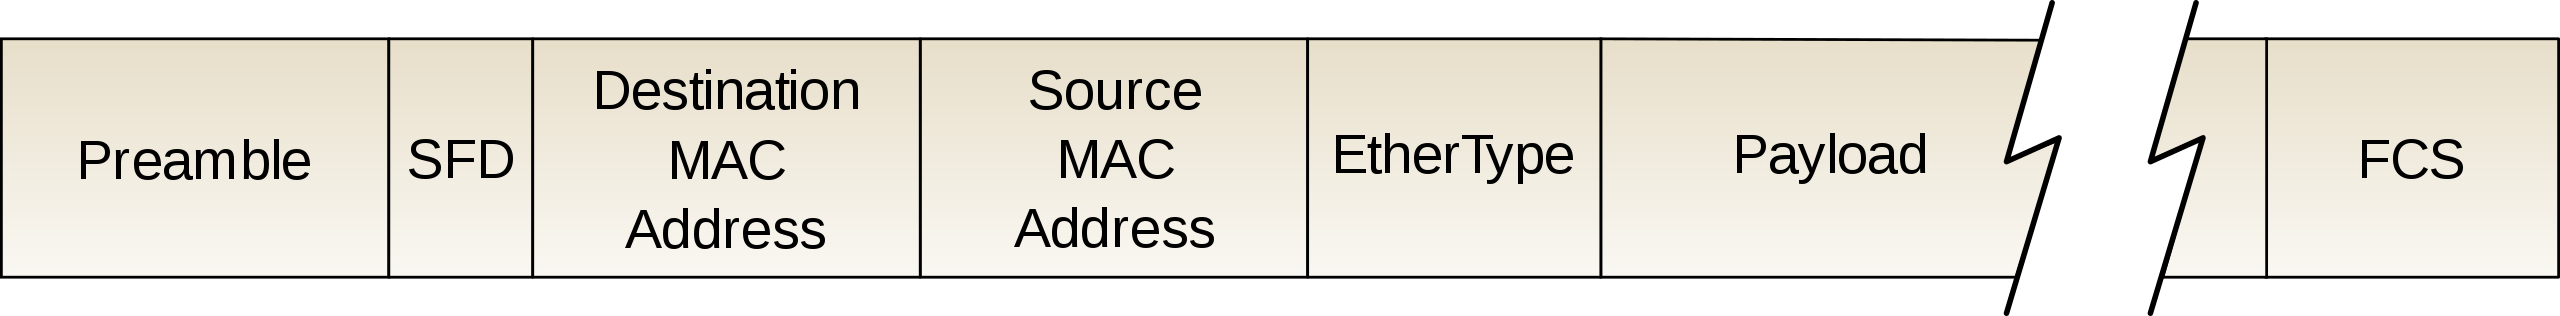
\includegraphics[width=\textwidth]{images/Ethernet_frame.png}
    \caption{An Ethernet frame inside an Ethernet packet, with SFD marking the end of the packet preamble and indicating the beginning of the frame}
    \label{fig:ethernet-frame}
\end{figure}


\Vref{fig:ethernet-frame} toont de velden in een Ethernet frame.
Eerst komen de \emph{preamble} en de \emph{start of frame delimiter} (SFD).
Deze dienen om het kloksignaal van de ontvanger af te stemmen op het kloksignaal van de zender zodat beide machines weten hoe lang het signaal van een 0 of een 1 duurt.

Hierna begint het eigenlijke Ethernet frame met het destination MAC-adres, gevolgd door het MAC-adres van de zender.
De \emph{EtherType} vertelt de ontvanger wat voor data er wordt verstuurd.
Enkele voorbeelden van geldige EtherTypes worden gegeven in \vref{tab:ethertype}.
Hierna komt de eigenlijke data of de \emph{payload} en ten slotte komt de \emph{frame check sequence} (FCS).
Dit is een code die gebruikt wordt om te detecteren of er fouten in het frame zitten.
Als het frame corrupt is, wordt deze gewoon verwijderd.
De ontvanger verwittigt de zender van het frame niet dat het frame niet goed is aangekomen.

\begin{table}[htp]
    \centering
    \begin{tabular}{ll}
    \textit{EtherType} & \textit{protocol} \\[1ex]
    0x0800 & IPv4 \\
    0x0806 & address resolution protocol (ARP) \\
    0x8100 & VLAN-tagged frame \\
    0x86DD & IPv6 \\
    \end{tabular}
    \caption{Enkele mogelijke waarden van de EtherType in een Ethernet frame}
    \label{tab:ethertype}
\end{table}


\section{Ethernetswitches}

Een Ethernetswitch ziet er niet anders uit dan een hub.
Een hub werkt echter heel anders dan een switch.
De interfaces van een hub zijn rechtstreeks met elkaar verbonden door middel van koperdraadjes zodat een elektrisch signaal dat binnenkomt op een van de interfaces, doorgestuurd wordt naar alle andere interfaces van de hub.
Een hub bevat geen intelligentie en kan niet geconfigureerd worden.

Een switch daarentegen is een toestel met heel wat intelligentie.
Er bestaan twee soorten switches: \emph{managed} en \emph{unmanaged} switches.
Unmanaged switches hebben de nodige intelligentie maar kunnen verder niet geconfigureerd worden.
Managed switches daarentegen beschikken over een volledig besturingssysteem en kunnen over zeer veel geavanceerde features beschikken.

\Vref{fig:ethernetswitch} toont een Juniper switch met 48~poorten of interfaces.
Rechts onder de display bevinden zich nog vier ``gaten'' in de switch.
Dit zijn sloten waar SFP-modules geplaatst kunnen worden (zie \vref{sec:sfp-modules}).

\begin{figure}
    \centering
    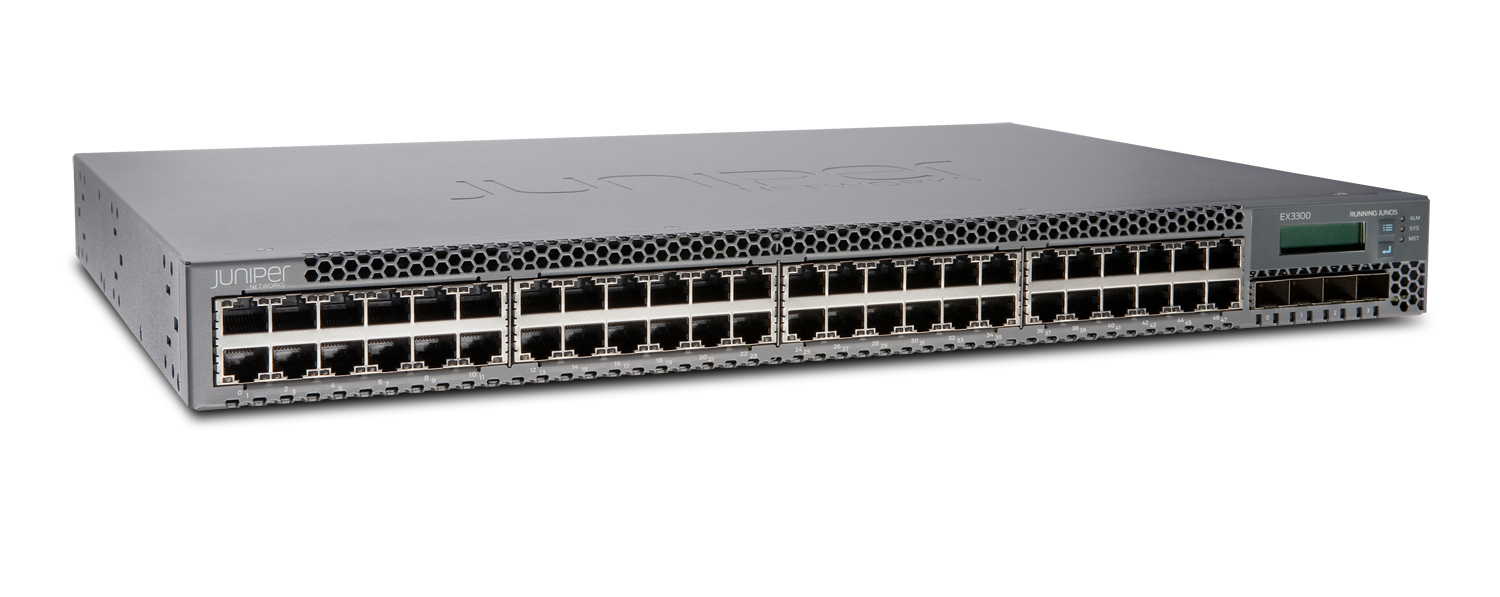
\includegraphics[width=\textwidth]{images/ethernetswitch.jpg}
    \caption{Een Ethernetswitch met 48 poorten en 4 openingen voor SFP-modules}
    \label{fig:ethernetswitch}
\end{figure}


In \vref{fig:simple-lan} zijn drie computers met elkaar verbonden via een switch.
Computer~1 wil communiceren met computer~2.
We gaan er even van uit dat beide computers elkaars IP-adres en MAC-adres kennen.
Als de switch de eerste frame ontvangt van computer~1, weet het nog niets over het netwerk of de toestellen die verbonden zijn met de switch, dus stuurt het het frame via alle interfaces naar buiten.
Computers~2 en~3 ontvangen dus dit eerste frame.
Computer~3 ziet het destination MAC-adres van het frame en, omdat dit niet zijn MAC-adres is, gooit het frame weg.
Computer~2 herkent wel zijn eigen MAC-adres in het frame en verwerkt de inhoud en stuurt uiteindelijk een antwoord terug.

De switch stuurt niet alleen het frame aan alle interfaces naar buiten, maar maakt ook notitie van het source MAC-adres en noteert dit in de MAC-tabel samen met de interface waarop hij het MAC-adres geleerd heeft.
\begin{center}
\begin{tabular}{cc}
\textit{MAC-adres} & \textit{interface} \\[1ex]
0200.aaaa.0001 & fa0/1\\
\end{tabular}
\end{center}
Als computer~2 nu een antwoord stuurt naar computer~1, komt dit frame aan op fa0/2 van de switch.
Weer noteert de switch het source MAC-adres in de MAC-tabel samen met de interface waarop de switch het frame ontvangt.
Vervolgens zoekt de switch het destination MAC-adres op in de MAC-tabel, vindt de bijhorende interface, en verstuurt het frame enkel langs deze interface naar buiten.
Computer~3 ziet dit antwoord -- en alle verder communicatie tussen computers~1 en~2 -- niet meer.

\begin{figure}
    \centering
    \documentclass[tikz]{standalone}
\usepackage{ifthen}
\usepackage{contour}
%%
%% Medtronic color palette
%%

\usepackage{xcolor}

% Primary blue color palette
\definecolor{mdtnavyblue}{cmyk}{1,.94,.47,.43}
\definecolor{mdtmedtronicblue}{cmyk}{.99,.74,.17,.04}
\definecolor{mdtcobaltblue}{cmyk}{.81,.35,0,0}
\definecolor{mdtmediumblue}{cmyk}{.73,.12,0,0}
\definecolor{mdtskyblue}{cmyk}{.55,.04,.04,0}
\definecolor{mdtlightblue}{cmyk}{.29,.05,.05,0}

% Primary neutral color palette
\definecolor{mdtcharcoal}{rgb}{.83,.86,.90}
\definecolor{mdtbluegray}{cmyk}{.68,.40,.28,.08}
\definecolor{mdtdarkgray}{cmyk}{0,0,0,.55}
\definecolor{mdtlightgray}{cmyk}{0,0,0,.30}
\definecolor{mdtpalegray}{cmyk}{.08,.06,.06,0}

% Accent colors
\definecolor{mdtyellow}{cmyk}{0,.18,.93,0}
\definecolor{mdtlightorange}{cmyk}{.02,.38,.96,0}
\definecolor{mdtorange}{cmyk}{.04,.78,1,0}
\definecolor{mdtpurple}{cmyk}{.38,.98,0,0}
\definecolor{mdtgreen}{cmyk}{.57,.02,1,0}
\definecolor{mdtturquoise}{cmyk}{.70,0,.38,0}

% TikZ/PGF
\usepackage{tikz}
\usetikzlibrary{backgrounds}
\usetikzlibrary{calc}
\usetikzlibrary{decorations.pathreplacing}
\usetikzlibrary{fit}
\usetikzlibrary{matrix}
\usetikzlibrary{patterns}
\usetikzlibrary{positioning}
\usetikzlibrary{shapes.geometric}
\usetikzlibrary{arrows}

%%
%% Styles
%%

% Network nodes
\tikzset{network node image/.style={
                inner sep=0mm,
                %anchor=south west
                }}
\tikzset{network node/.style={
                network node image,
                thick,
                text=mdtmedtronicblue,
                draw=mdtmedtronicblue,
                fill=white,
                minimum size=10mm}}
\tikzset{network node circle/.style={
                network node,
                circle}}
\tikzset{network node square/.style={
                network node,
                rectangle,
                rounded corners}}
\tikzset{network node rectangle/.style={
                network node,
                rectangle,
                minimum height=15mm,
                rounded corners}}
\tikzset{server rack/.style={
                align=left,
                text width=8mm,
                inner sep=0pt,
                anchor=north west,
                minimum height=7.5mm-.8pt,
                minimum width=10.7mm-.8pt,
                thick,
                text=mdtmedtronicblue,
                draw=mdtmedtronicblue,
                fill=white}}
\tikzset{network rack/.style={
                align=left,
                text width=9.3mm,
                inner sep=0pt,
                anchor=north west,
                minimum height=7.5mm-.8pt,
                minimum width=12mm-.8pt,
                %minimum height=7.5mm,
                %minimum width=12mm,
                thick,
                text=mdtmedtronicblue,
                draw=mdtmedtronicblue,
                fill=white}}
\tikzset{patch rack/.style={
                align=left,
                text width=9.3mm,
                inner sep=0pt,
                anchor=north west,
                minimum height=7.5mm-.8pt,
                minimum width=12mm-.8pt,
                thick,
                text=mdtmedtronicblue,
                draw=mdtmedtronicblue,
                fill=white}}

% Labels
\tikzset{interface label/.style={
                font=\footnotesize,
                inner sep=2pt},
                fill=white}
\tikzset{node label/.style={
                font=\small,
                align=center,
                inner sep=2pt,
                thick,
                rounded corners}}


% Floor tiles
\newcommand{\dcfloortiles}[2]{%
    \draw[step=6mm,gray,very thin] (0,0) grid ($.6*(#1,#2)$);
}
\newcommand{\dccoldaisle}[2]{%
    \draw[pattern=north west lines, pattern color=mdtlightgray] ($.6*(#1)-(.6,.6)$) rectangle ($.6*(#1)+.6*(#2)-(.6,.6)$);
}
% Markings for different types of racks
\newcommand{\caserack}[1]{%
    \draw[very thick,mdtorange] ($(#1.north east)-(.1,.1)$) -- ($(#1.south east)+(-.1,.1)$);
}
\newcommand{\storagerack}[1]{%
    \draw[very thick,mdtgreen] ($(#1.north east)-(.2,.1)$) -- ($(#1.south east)+(-.2,.1)$);
}
\newcommand{\networkrack}[1]{%
    \draw[very thick,mdtmediumblue] ($(#1.north east)-(.15,.1)$) -- ($(#1.south east)+(-.15,.1)$);
}
\newcommand{\mitgrack}[1]{%
    \draw[very thick,mdtpurple] ($(#1.north east)-(.25,.1)$) -- ($(#1.south east)+(-.25,.1)$);
}
\newcommand{\unixrack}[1]{%
    \draw[very thick,mdtdarkgray] ($(#1.north east)-(.3,.1)$) -- ($(#1.south east)+(-.3,.1)$);
}
\newcommand{\computerack}[1]{%
    \draw[very thick,mdtturquoise] ($(#1.north east)-(.35,.1)$) -- ($(#1.south east)+(-.35,.1)$);
}
\newcommand{\racklabels}[1]{%
    \matrix (racklabels) at (#1) [matrix of nodes,
        nodes={
            anchor=west,
            align=left
            }
        ] {
            |[mdtorange]| CASE \\
            |[mdtturquoise]| Compute (CORE) \\
            |[mdtpurple]| MITG \\
            |[mdtmediumblue]| Network \\
            |[mdtgreen]| Storage \\
            |[mdtdarkgray]| UNIX \\
    };
}
%
% layers.tex
%
% This document contains code to hide a PGF layer if so desired,
% e.g. you can hide the layer with all the labels on it.
%

% Define the layers to be used
\pgfdeclarelayer{connections}
\pgfdeclarelayer{interfaces}
\pgfdeclarelayer{hostnames}
\pgfdeclarelayer{labels}
\pgfdeclarelayer{arrows}

% Make the background white so we can hide the labels by swapping the order of the layers
\tikzset{show background rectangle,background rectangle/.style={rounded corners,fill=white}}

% \showalllayers - Show the nodes, connections, and detailed labels, including interface labels
% The left most layer is the bottom layer; everything left from the background will be hidden.
\newcommand\showalllayers{      \pgfsetlayers{hostnames,arrows,background,connections,main,interfaces,labels}}
\newcommand\showarrows{         \pgfsetlayers{hostnames,background,connections,main,interfaces,labels,arrows}}
% \hidelabels - Show only the nodes and the connections
\newcommand\hidelabels{         \pgfsetlayers{hostnames,arrows,interfaces,labels,background,connections,main}}
% \hideinterfaces - Hide only the interface labels
\newcommand\hideinterfaces{     \pgfsetlayers{hostnames,arrows,interfaces,background,connections,main,labels}}
% \showonlyhostnames - Hide everything but show the hostnames only
\newcommand\showonlyhostnames{  \pgfsetlayers{arrows,interfaces,labels,background,connections,main,hostnames}}
\newcommand\showhostnamesinterfaces{ \pgfsetlayers{arrows,labels,background,connections,main,hostnames,interfaces}}
% Default setting is to show all layers
\showalllayers
%
% connections.tex
%
% This document contains all the commands needed to create connections between
% different network nodes, e.g.
%  - a normal connection, with our without labels.
%  - a vPC connection between 3 or 4 nodes.
%

%
% Syntax:
% \connect[<color>]{<node1>}{<intf1>}{<node2>}{<intf2>}
\newcommand{\connect}[5][black]{

    % Save the coordinates for the interface labels
    \path (#2) -- (#4) coordinate[very near start] (i1) coordinate[midway] (im) coordinate[very near end] (i2);
    
    % Draw the connection between the two devices on the correct layer.
    \begin{pgfonlayer}{connections}
      \draw[color=#1] (#2) -- (#4);
    \end{pgfonlayer}
    
    % Draw the interface labels on the correct layer.
    \begin{pgfonlayer}{interfaces}
        \ifthenelse{\equal{#3}{}}{}{\node[interface label,fill=white] at (i1) {\contour{white}{#3}};}
        \ifthenelse{\equal{#5}{}}{}{\node[interface label,fill=white] at (i2) {\contour{white}{#5}};}
    \end{pgfonlayer}
    
    %\ifthenelse{\equal{#5}{}}{
    %    % Parameter 5 is empty:
    %    \ifthenelse{\equal{#3}{}}{
    %        % Parameter 3 is empty: no interfaces have been given.
    %        \draw[color=#1] (#2) -- (#4);
    %    }{
    %        % Both devices share the same interface name.
    %        \draw[color=#1] (#2) -- (#4)
    %            node [midway,interface] {#3};
    %    }
    %}{
    %    % Parameter 5 is not empty: both interfaces are given.
    %    \draw[color=#1] (#2) -- (#4)
    %        node [on background layer,near start,interface] {#3}
    %        node [near end,interface] {#5};
    %}
}

%
% Syntax:
% \connectClusters[<straight/cross>]{cluster1}{cluster2}
\newcommand{\connectClusters}[3][S]{
    \message{connectClusters 2-1: #2-1^^J}
    \message{connectClusters 2-2: #2-2^^J}
    \message{connectClusters 3-1: #3-1^^J}
    \message{connectClusters 3-2: #3-2^^J}
    \ifthenelse{\equal{#1}{S}}{
        \connect{#2-1}{}{#3-1}{}
        \connect{#2-2}{}{#3-2}{}
    }{
        \connect{#2-1}{}{#3-2}{}
        \connect{#2-2}{}{#3-1}{}
    }
}

%
% Syntax:
% \arrowcoords[<position>]{<coordinates start>}{<coordinates end>}{<text>}
\newcommand{\arrowcoords}[4][midway]{
    \draw[mdtgreen, arrows={-latex'}, shorten <= 0.25cm, shorten >= 0.25cm, very thick, distance=2cm] (#2) to[out=230,in=170] (#3) node[#1] {#4};
}

%
%
%

\def\iconset{3015}


%
% Display only the icons
%
% Syntax: \icon<type>{<hostname>}{<coordinates>}
%

\newcommand{\iconcloud}[2]{
    \node[network node image] (#1) at (#2) {
\includegraphics[width=30mm]{images//cloud.png}};
    \node at ([yshift=-2mm]#2) {#1};
}
\newcommand{\iconfirewall}[2]{
    \ifthenelse{\equal{\iconset}{basic}}{
        \node[network node circle,draw=mdtorange] (#1) at (#2) {FW};
    }{
        \node[network node image] (#1) at (#2) {
\includegraphics[width=10mm]{images/\iconset/firewall.eps}};
    }
}
\newcommand{\iconips}[2]{
    \ifthenelse{\equal{\iconset}{basic}}{
        \node[network node square] (#1) at (#2) {IPS};
    }{
        \node[network node image] (#1) at (#2) {\includegraphics[width=10mm]{images/\iconset/ips.eps}};
    }
}
\newcommand{\iconrouter}[2]{
    \ifthenelse{\equal{\iconset}{basic}}{
        \node[network node circle] (#1) at (#2) {RTR};
    }{
        \node[network node image] (#1) at (#2) {
\includegraphics[width=10mm]{images/\iconset/router.eps}};
    }
    \message{iconrouter: #1^^J}
}
\newcommand{\iconswitch}[2]{
    \ifthenelse{\equal{\iconset}{basic}}{
        \node[network node square] (#1) at (#2) {SW};
    }{
        \node[network node image] (#1) at (#2) {
\includegraphics[width=13mm]{images/\iconset/switch.eps}};
    }
}
\newcommand{\icondistswitch}[2]{
    \ifthenelse{\equal{\iconset}{basic}}{
        \node[network node square] (#1) at (#2) {SW};
    }{
        \node[network node image] (#1) at (#2) {\includegraphics[width=13mm]{images/\iconset/l3switch.eps}};
    }
}
\newcommand{\iconcoreswitch}[2]{
    \ifthenelse{\equal{\iconset}{basic}}{
        \node[network node square] (#1) at (#2) {SW};
    }{
        \node[network node image] (#1) at (#2) {\includegraphics[width=13mm]{images/\iconset/coreswitch.eps}};
    }
}
\newcommand{\iconhost}[2]{
   \ifthenelse{\equal{\iconset}{basic}}{
      \node[network node square] (#1) at (#2) {PC};
   }{
      \node[network node square] (#1) at (#2) {PC};
   }
}



%
% Display the node: icon + labels
%
%
% Syntax: \node<type>[<label position>]{<name>}{<coordinates>}{<type>}{<IP address>}
%
% Where:
%  - <label position> : top, bottom, left, right (default)
%  - <type> : hardware type, e.g. Catalyst 3850
%

\newcommand{\nodecloud}[5][right]{
    \iconcloud{#2}{#3}
}
\newcommand{\nodefirewall}[5][right]{
    \iconfirewall{#2}{#3}
    \nodelabel[#1]{#3}{#2}{#4}{#5}
}
\newcommand{\nodeips}[5][right]{
    \iconips{#2}{#3}
    \nodelabel[#1]{#3}{#2}{#4}{#5}
}
\newcommand{\noderouter}[5][right]{
    \iconrouter{#2}{#3}
    \nodelabel[#1]{#3}{#2}{#4}{#5}
}
\newcommand{\nodedistswitch}[5][right]{
    \icondistswitch{#2}{#3}
    \nodelabel[#1]{#3}{#2}{#4}{#5}
}
\newcommand{\nodeswitch}[5][right]{    
    \iconswitch{#2}{#3}
    \nodelabel[#1]{#3}{#2}{#4}{#5}
}
\newcommand{\nodecoreswitch}[5][right]{    
    \iconcoreswitch{#2}{#3}
    \nodelabel[#1]{$(#3)-(0,.4)$}{#2}{#4}{#5}
}
\newcommand{\nodehost}[5][right]{
   \iconhost{#2}{#3}
   \nodelabel[#1]{#3}{#2}{#4}{#5}
}



%
% Clusters of nodes
%
% Syntax: \cluster<type>[<label position>]{<name>}{<coordinates>}{<type>}{<IP address>}
%

\newcommand{\clustercloud}[3][bottom]{
    \draw[network node,draw=mdtpurple,fill=mdtpalegray] (#3) ellipse (15mm and 10mm);
    \node (#2) at (#3) {#2};
    \ifthenelse{\equal{#1}{top}}{
        \coordinate (a) at ($(#3)-(10mm,-7mm)$);
        \coordinate (b) at ($(#3)+(10mm,7mm)$);
    }{
        \coordinate (a) at ($(#3)-(10mm,7mm)$);
        \coordinate (b) at ($(#3)+(10mm,-7mm)$);
    }
    \message{clustercloud: #2-1^^J}
    \iconrouter{#2-1}{a}
    \message{clustercloud: #2-2^^J}
    \iconrouter{#2-2}{b}
}

\newcommand{\clusterfirewall}[5][bottom]{
    \coordinate (left) at ($(#3)-(1,0)$);
    \coordinate (right) at ($(#3)+(1,0)$);
    \iconfirewall{#2-1}{left}
    \iconfirewall{#2-2}{right}
    
    \begin{pgfonlayer}{connections}
        \node (#2) [draw=mdtmedtronicblue,rounded corners,inner sep=2mm,dashed,fit=(#2-1) (#2-2)] {};
    \end{pgfonlayer}
    \connect{#2-1}{}{#2-2}{}
    
    \nodelabel[#1]{#3}{#2}{#4}{#5}
}




%
% Syntax:
% \nodelabel[<position>]{<coordinates>}{<hostname>}{<type>}{<IP address>}
\newcommand{\nodelabel}[5][right]{
    \def\text{\contour{white}{\textbf{#3}}\\\contour{white}{\emph{#4}}\\\contour{white}{#5}}
    \begin{pgfonlayer}{labels}
    
    % On the right
    \ifthenelse{\equal{#1}{right}}{
        %\node[node label,anchor=west] at ($(#2)+(1,0)$) {\contour{white}{\textbf{#3}\\\emph{#4}\\#5}};
        \node[node label,anchor=west] at ($(#2)+(1,0)$) {\text};
        
    % On the left
    }{\ifthenelse{\equal{#1}{left}}{
        \node[node label,anchor=east] at ($(#2)-(1,0)$) {\text};
    
    % At the top
    }{\ifthenelse{\equal{#1}{top}}{
        \node[node label,anchor=south] at ($(#2)+(0,1)$) {\text};
    
    % At the bottom
    }{\ifthenelse{\equal{#1}{bottom}}{
        \node[node label,anchor=north] at ($(#2)-(0,1)$) {\text};
    
    }{}}}}
    
    \end{pgfonlayer}
    
    \begin{pgfonlayer}{hostnames}
        \node[node label,anchor=north] at ($(#2)-(0,.6)$) {\contour{white}{#3}};
    \end{pgfonlayer}
}

%
% Syntax:
% \vlaninformationR[<xshift>]{<node name>}{<relative location>}
%\newcommand{\vlaninformationR}[4][5cm]{
%    \matrix (#2) [matrix of nodes,
%        right=of #3,
%        xshift=#1,
%        left delimiter=\{,
%        nodes={
%            anchor=west,
%            align=left
%            }
%        ] {
%            #4
%    };
%}
\begin{document}
\begin{tikzpicture}[framed]
\def\iconset{basic}
%\showhostnamesinterfaces
\nodeswitch[bottom]{switch}{3,0}{Cisco 2960}{}
\nodehost[left]{pc 1}{0,0}{FreeBSD}{0200.aaaa.0001}
\nodehost{pc 2}{6,0}{FreeBSD}{0200.aaaa.0002}
\nodehost{pc 3}{3,3}{Linux}{0200.aaaa.0003}
\connect{switch}{fa0/1}{pc 1}{em0}
\connect{switch}{fa0/2}{pc 2}{em0}
\connect{switch}{fa0/3}{pc 3}{eth0}


\end{tikzpicture}
\end{document}
    \caption{Een eenvoudig netwerk met twee computers die met elkaar verbonden zijn via een switch}
    \label{fig:simple-lan}
\end{figure}

Een MAC-adres kan slechts aan één interface gekoppeld zijn.
Als de switch een MAC-adres dat het al kent, opnieuw leert via een andere interface, dan update het de bestaande entry in de MAC-tabel door de oude interface te vervangen door de nieuwe interface.

Het is wel mogelijk dat meerdere MAC-adressen op dezelfde interface geleerd worden.
Dit is mogelijk als een computer met meerdere virtuele machines, verbonden wordt met de switch.
Elke virtuele machine heeft immers een eigen MAC-adres.
Het is ook mogelijk meerdere MAC-adressen te leren op een interface als deze interface met een andere switch verbindt.
De eerste switch leert dan de MAC-adressen van alle computers die verbinden met de tweede switch via deze interface.


\section{Lussen in het netwerk}
\label{sec:stp}

Als één switch niet meer voldoende is om alle computers en printers met elkaar te verbinden, verbinden we een tweede switch met de eerste switch.
Als beide switch niet meer voldoende zijn, kunnen we nog een derde switch verbinden met het netwerk, en vervolgens nog een vierde en vijfde switch (zie \vref{fig:daisy-chain}).
Een dergelijk netwerk kan lang goed functioneren.
Tot op een dag bijvoorbeeld switch~2 kapot gaat en alle computers die met switches~3 tot en met~5 verbonden zijn, geen Internetconnectiviteit meer hebben.
Maar dit is eenvoudig op te lossen.
We verbinden switch~1 snel met switch~3 en de connectiviteit is hersteld.


\begin{figure}
    \centering
    \documentclass[tikz]{standalone}
\usepackage{ifthen}
\usepackage{contour}
%%
%% Medtronic color palette
%%

\usepackage{xcolor}

% Primary blue color palette
\definecolor{mdtnavyblue}{cmyk}{1,.94,.47,.43}
\definecolor{mdtmedtronicblue}{cmyk}{.99,.74,.17,.04}
\definecolor{mdtcobaltblue}{cmyk}{.81,.35,0,0}
\definecolor{mdtmediumblue}{cmyk}{.73,.12,0,0}
\definecolor{mdtskyblue}{cmyk}{.55,.04,.04,0}
\definecolor{mdtlightblue}{cmyk}{.29,.05,.05,0}

% Primary neutral color palette
\definecolor{mdtcharcoal}{rgb}{.83,.86,.90}
\definecolor{mdtbluegray}{cmyk}{.68,.40,.28,.08}
\definecolor{mdtdarkgray}{cmyk}{0,0,0,.55}
\definecolor{mdtlightgray}{cmyk}{0,0,0,.30}
\definecolor{mdtpalegray}{cmyk}{.08,.06,.06,0}

% Accent colors
\definecolor{mdtyellow}{cmyk}{0,.18,.93,0}
\definecolor{mdtlightorange}{cmyk}{.02,.38,.96,0}
\definecolor{mdtorange}{cmyk}{.04,.78,1,0}
\definecolor{mdtpurple}{cmyk}{.38,.98,0,0}
\definecolor{mdtgreen}{cmyk}{.57,.02,1,0}
\definecolor{mdtturquoise}{cmyk}{.70,0,.38,0}

% TikZ/PGF
\usepackage{tikz}
\usetikzlibrary{backgrounds}
\usetikzlibrary{calc}
\usetikzlibrary{decorations.pathreplacing}
\usetikzlibrary{fit}
\usetikzlibrary{matrix}
\usetikzlibrary{patterns}
\usetikzlibrary{positioning}
\usetikzlibrary{shapes.geometric}
\usetikzlibrary{arrows}

%%
%% Styles
%%

% Network nodes
\tikzset{network node image/.style={
                inner sep=0mm,
                %anchor=south west
                }}
\tikzset{network node/.style={
                network node image,
                thick,
                text=mdtmedtronicblue,
                draw=mdtmedtronicblue,
                fill=white,
                minimum size=10mm}}
\tikzset{network node circle/.style={
                network node,
                circle}}
\tikzset{network node square/.style={
                network node,
                rectangle,
                rounded corners}}
\tikzset{network node rectangle/.style={
                network node,
                rectangle,
                minimum height=15mm,
                rounded corners}}
\tikzset{server rack/.style={
                align=left,
                text width=8mm,
                inner sep=0pt,
                anchor=north west,
                minimum height=7.5mm-.8pt,
                minimum width=10.7mm-.8pt,
                thick,
                text=mdtmedtronicblue,
                draw=mdtmedtronicblue,
                fill=white}}
\tikzset{network rack/.style={
                align=left,
                text width=9.3mm,
                inner sep=0pt,
                anchor=north west,
                minimum height=7.5mm-.8pt,
                minimum width=12mm-.8pt,
                %minimum height=7.5mm,
                %minimum width=12mm,
                thick,
                text=mdtmedtronicblue,
                draw=mdtmedtronicblue,
                fill=white}}
\tikzset{patch rack/.style={
                align=left,
                text width=9.3mm,
                inner sep=0pt,
                anchor=north west,
                minimum height=7.5mm-.8pt,
                minimum width=12mm-.8pt,
                thick,
                text=mdtmedtronicblue,
                draw=mdtmedtronicblue,
                fill=white}}

% Labels
\tikzset{interface label/.style={
                font=\footnotesize,
                inner sep=2pt},
                fill=white}
\tikzset{node label/.style={
                font=\small,
                align=center,
                inner sep=2pt,
                thick,
                rounded corners}}


% Floor tiles
\newcommand{\dcfloortiles}[2]{%
    \draw[step=6mm,gray,very thin] (0,0) grid ($.6*(#1,#2)$);
}
\newcommand{\dccoldaisle}[2]{%
    \draw[pattern=north west lines, pattern color=mdtlightgray] ($.6*(#1)-(.6,.6)$) rectangle ($.6*(#1)+.6*(#2)-(.6,.6)$);
}
% Markings for different types of racks
\newcommand{\caserack}[1]{%
    \draw[very thick,mdtorange] ($(#1.north east)-(.1,.1)$) -- ($(#1.south east)+(-.1,.1)$);
}
\newcommand{\storagerack}[1]{%
    \draw[very thick,mdtgreen] ($(#1.north east)-(.2,.1)$) -- ($(#1.south east)+(-.2,.1)$);
}
\newcommand{\networkrack}[1]{%
    \draw[very thick,mdtmediumblue] ($(#1.north east)-(.15,.1)$) -- ($(#1.south east)+(-.15,.1)$);
}
\newcommand{\mitgrack}[1]{%
    \draw[very thick,mdtpurple] ($(#1.north east)-(.25,.1)$) -- ($(#1.south east)+(-.25,.1)$);
}
\newcommand{\unixrack}[1]{%
    \draw[very thick,mdtdarkgray] ($(#1.north east)-(.3,.1)$) -- ($(#1.south east)+(-.3,.1)$);
}
\newcommand{\computerack}[1]{%
    \draw[very thick,mdtturquoise] ($(#1.north east)-(.35,.1)$) -- ($(#1.south east)+(-.35,.1)$);
}
\newcommand{\racklabels}[1]{%
    \matrix (racklabels) at (#1) [matrix of nodes,
        nodes={
            anchor=west,
            align=left
            }
        ] {
            |[mdtorange]| CASE \\
            |[mdtturquoise]| Compute (CORE) \\
            |[mdtpurple]| MITG \\
            |[mdtmediumblue]| Network \\
            |[mdtgreen]| Storage \\
            |[mdtdarkgray]| UNIX \\
    };
}
%
% layers.tex
%
% This document contains code to hide a PGF layer if so desired,
% e.g. you can hide the layer with all the labels on it.
%

% Define the layers to be used
\pgfdeclarelayer{connections}
\pgfdeclarelayer{interfaces}
\pgfdeclarelayer{hostnames}
\pgfdeclarelayer{labels}
\pgfdeclarelayer{arrows}

% Make the background white so we can hide the labels by swapping the order of the layers
\tikzset{show background rectangle,background rectangle/.style={rounded corners,fill=white}}

% \showalllayers - Show the nodes, connections, and detailed labels, including interface labels
% The left most layer is the bottom layer; everything left from the background will be hidden.
\newcommand\showalllayers{      \pgfsetlayers{hostnames,arrows,background,connections,main,interfaces,labels}}
\newcommand\showarrows{         \pgfsetlayers{hostnames,background,connections,main,interfaces,labels,arrows}}
% \hidelabels - Show only the nodes and the connections
\newcommand\hidelabels{         \pgfsetlayers{hostnames,arrows,interfaces,labels,background,connections,main}}
% \hideinterfaces - Hide only the interface labels
\newcommand\hideinterfaces{     \pgfsetlayers{hostnames,arrows,interfaces,background,connections,main,labels}}
% \showonlyhostnames - Hide everything but show the hostnames only
\newcommand\showonlyhostnames{  \pgfsetlayers{arrows,interfaces,labels,background,connections,main,hostnames}}
\newcommand\showhostnamesinterfaces{ \pgfsetlayers{arrows,labels,background,connections,main,hostnames,interfaces}}
% Default setting is to show all layers
\showalllayers
%
% connections.tex
%
% This document contains all the commands needed to create connections between
% different network nodes, e.g.
%  - a normal connection, with our without labels.
%  - a vPC connection between 3 or 4 nodes.
%

%
% Syntax:
% \connect[<color>]{<node1>}{<intf1>}{<node2>}{<intf2>}
\newcommand{\connect}[5][black]{

    % Save the coordinates for the interface labels
    \path (#2) -- (#4) coordinate[very near start] (i1) coordinate[midway] (im) coordinate[very near end] (i2);
    
    % Draw the connection between the two devices on the correct layer.
    \begin{pgfonlayer}{connections}
      \draw[color=#1] (#2) -- (#4);
    \end{pgfonlayer}
    
    % Draw the interface labels on the correct layer.
    \begin{pgfonlayer}{interfaces}
        \ifthenelse{\equal{#3}{}}{}{\node[interface label,fill=white] at (i1) {\contour{white}{#3}};}
        \ifthenelse{\equal{#5}{}}{}{\node[interface label,fill=white] at (i2) {\contour{white}{#5}};}
    \end{pgfonlayer}
    
    %\ifthenelse{\equal{#5}{}}{
    %    % Parameter 5 is empty:
    %    \ifthenelse{\equal{#3}{}}{
    %        % Parameter 3 is empty: no interfaces have been given.
    %        \draw[color=#1] (#2) -- (#4);
    %    }{
    %        % Both devices share the same interface name.
    %        \draw[color=#1] (#2) -- (#4)
    %            node [midway,interface] {#3};
    %    }
    %}{
    %    % Parameter 5 is not empty: both interfaces are given.
    %    \draw[color=#1] (#2) -- (#4)
    %        node [on background layer,near start,interface] {#3}
    %        node [near end,interface] {#5};
    %}
}

%
% Syntax:
% \connectClusters[<straight/cross>]{cluster1}{cluster2}
\newcommand{\connectClusters}[3][S]{
    \message{connectClusters 2-1: #2-1^^J}
    \message{connectClusters 2-2: #2-2^^J}
    \message{connectClusters 3-1: #3-1^^J}
    \message{connectClusters 3-2: #3-2^^J}
    \ifthenelse{\equal{#1}{S}}{
        \connect{#2-1}{}{#3-1}{}
        \connect{#2-2}{}{#3-2}{}
    }{
        \connect{#2-1}{}{#3-2}{}
        \connect{#2-2}{}{#3-1}{}
    }
}

%
% Syntax:
% \arrowcoords[<position>]{<coordinates start>}{<coordinates end>}{<text>}
\newcommand{\arrowcoords}[4][midway]{
    \draw[mdtgreen, arrows={-latex'}, shorten <= 0.25cm, shorten >= 0.25cm, very thick, distance=2cm] (#2) to[out=230,in=170] (#3) node[#1] {#4};
}

%
%
%

\def\iconset{3015}


%
% Display only the icons
%
% Syntax: \icon<type>{<hostname>}{<coordinates>}
%

\newcommand{\iconcloud}[2]{
    \node[network node image] (#1) at (#2) {
\includegraphics[width=30mm]{images//cloud.png}};
    \node at ([yshift=-2mm]#2) {#1};
}
\newcommand{\iconfirewall}[2]{
    \ifthenelse{\equal{\iconset}{basic}}{
        \node[network node circle,draw=mdtorange] (#1) at (#2) {FW};
    }{
        \node[network node image] (#1) at (#2) {
\includegraphics[width=10mm]{images/\iconset/firewall.eps}};
    }
}
\newcommand{\iconips}[2]{
    \ifthenelse{\equal{\iconset}{basic}}{
        \node[network node square] (#1) at (#2) {IPS};
    }{
        \node[network node image] (#1) at (#2) {\includegraphics[width=10mm]{images/\iconset/ips.eps}};
    }
}
\newcommand{\iconrouter}[2]{
    \ifthenelse{\equal{\iconset}{basic}}{
        \node[network node circle] (#1) at (#2) {RTR};
    }{
        \node[network node image] (#1) at (#2) {
\includegraphics[width=10mm]{images/\iconset/router.eps}};
    }
    \message{iconrouter: #1^^J}
}
\newcommand{\iconswitch}[2]{
    \ifthenelse{\equal{\iconset}{basic}}{
        \node[network node square] (#1) at (#2) {SW};
    }{
        \node[network node image] (#1) at (#2) {
\includegraphics[width=13mm]{images/\iconset/switch.eps}};
    }
}
\newcommand{\icondistswitch}[2]{
    \ifthenelse{\equal{\iconset}{basic}}{
        \node[network node square] (#1) at (#2) {SW};
    }{
        \node[network node image] (#1) at (#2) {\includegraphics[width=13mm]{images/\iconset/l3switch.eps}};
    }
}
\newcommand{\iconcoreswitch}[2]{
    \ifthenelse{\equal{\iconset}{basic}}{
        \node[network node square] (#1) at (#2) {SW};
    }{
        \node[network node image] (#1) at (#2) {\includegraphics[width=13mm]{images/\iconset/coreswitch.eps}};
    }
}
\newcommand{\iconhost}[2]{
   \ifthenelse{\equal{\iconset}{basic}}{
      \node[network node square] (#1) at (#2) {PC};
   }{
      \node[network node square] (#1) at (#2) {PC};
   }
}



%
% Display the node: icon + labels
%
%
% Syntax: \node<type>[<label position>]{<name>}{<coordinates>}{<type>}{<IP address>}
%
% Where:
%  - <label position> : top, bottom, left, right (default)
%  - <type> : hardware type, e.g. Catalyst 3850
%

\newcommand{\nodecloud}[5][right]{
    \iconcloud{#2}{#3}
}
\newcommand{\nodefirewall}[5][right]{
    \iconfirewall{#2}{#3}
    \nodelabel[#1]{#3}{#2}{#4}{#5}
}
\newcommand{\nodeips}[5][right]{
    \iconips{#2}{#3}
    \nodelabel[#1]{#3}{#2}{#4}{#5}
}
\newcommand{\noderouter}[5][right]{
    \iconrouter{#2}{#3}
    \nodelabel[#1]{#3}{#2}{#4}{#5}
}
\newcommand{\nodedistswitch}[5][right]{
    \icondistswitch{#2}{#3}
    \nodelabel[#1]{#3}{#2}{#4}{#5}
}
\newcommand{\nodeswitch}[5][right]{    
    \iconswitch{#2}{#3}
    \nodelabel[#1]{#3}{#2}{#4}{#5}
}
\newcommand{\nodecoreswitch}[5][right]{    
    \iconcoreswitch{#2}{#3}
    \nodelabel[#1]{$(#3)-(0,.4)$}{#2}{#4}{#5}
}
\newcommand{\nodehost}[5][right]{
   \iconhost{#2}{#3}
   \nodelabel[#1]{#3}{#2}{#4}{#5}
}



%
% Clusters of nodes
%
% Syntax: \cluster<type>[<label position>]{<name>}{<coordinates>}{<type>}{<IP address>}
%

\newcommand{\clustercloud}[3][bottom]{
    \draw[network node,draw=mdtpurple,fill=mdtpalegray] (#3) ellipse (15mm and 10mm);
    \node (#2) at (#3) {#2};
    \ifthenelse{\equal{#1}{top}}{
        \coordinate (a) at ($(#3)-(10mm,-7mm)$);
        \coordinate (b) at ($(#3)+(10mm,7mm)$);
    }{
        \coordinate (a) at ($(#3)-(10mm,7mm)$);
        \coordinate (b) at ($(#3)+(10mm,-7mm)$);
    }
    \message{clustercloud: #2-1^^J}
    \iconrouter{#2-1}{a}
    \message{clustercloud: #2-2^^J}
    \iconrouter{#2-2}{b}
}

\newcommand{\clusterfirewall}[5][bottom]{
    \coordinate (left) at ($(#3)-(1,0)$);
    \coordinate (right) at ($(#3)+(1,0)$);
    \iconfirewall{#2-1}{left}
    \iconfirewall{#2-2}{right}
    
    \begin{pgfonlayer}{connections}
        \node (#2) [draw=mdtmedtronicblue,rounded corners,inner sep=2mm,dashed,fit=(#2-1) (#2-2)] {};
    \end{pgfonlayer}
    \connect{#2-1}{}{#2-2}{}
    
    \nodelabel[#1]{#3}{#2}{#4}{#5}
}




%
% Syntax:
% \nodelabel[<position>]{<coordinates>}{<hostname>}{<type>}{<IP address>}
\newcommand{\nodelabel}[5][right]{
    \def\text{\contour{white}{\textbf{#3}}\\\contour{white}{\emph{#4}}\\\contour{white}{#5}}
    \begin{pgfonlayer}{labels}
    
    % On the right
    \ifthenelse{\equal{#1}{right}}{
        %\node[node label,anchor=west] at ($(#2)+(1,0)$) {\contour{white}{\textbf{#3}\\\emph{#4}\\#5}};
        \node[node label,anchor=west] at ($(#2)+(1,0)$) {\text};
        
    % On the left
    }{\ifthenelse{\equal{#1}{left}}{
        \node[node label,anchor=east] at ($(#2)-(1,0)$) {\text};
    
    % At the top
    }{\ifthenelse{\equal{#1}{top}}{
        \node[node label,anchor=south] at ($(#2)+(0,1)$) {\text};
    
    % At the bottom
    }{\ifthenelse{\equal{#1}{bottom}}{
        \node[node label,anchor=north] at ($(#2)-(0,1)$) {\text};
    
    }{}}}}
    
    \end{pgfonlayer}
    
    \begin{pgfonlayer}{hostnames}
        \node[node label,anchor=north] at ($(#2)-(0,.6)$) {\contour{white}{#3}};
    \end{pgfonlayer}
}

%
% Syntax:
% \vlaninformationR[<xshift>]{<node name>}{<relative location>}
%\newcommand{\vlaninformationR}[4][5cm]{
%    \matrix (#2) [matrix of nodes,
%        right=of #3,
%        xshift=#1,
%        left delimiter=\{,
%        nodes={
%            anchor=west,
%            align=left
%            }
%        ] {
%            #4
%    };
%}
\begin{document}
\begin{tikzpicture}[framed]
\def\iconset{basic}
\nodecloud{Internet}{0,4}{}{}
\nodefirewall{firewall}{0,2}{}{}
\nodeswitch[bottom]{sw1}{0,0}{}{}
\nodeswitch[bottom]{sw2}{2,0}{}{}
\nodeswitch[bottom]{sw3}{4,0}{}{}
\nodeswitch[bottom]{sw4}{6,0}{}{}
\nodeswitch[bottom]{sw5}{8,0}{}{}
\connect{Internet}{}{firewall}{}
\connect{firewall}{}{sw1}{}
\connect{sw1}{}{sw2}{}
\connect{sw2}{}{sw3}{}
\connect{sw3}{}{sw4}{}
\connect{sw4}{}{sw5}{}
\end{tikzpicture}
\end{document}
    \caption{Meerdere switches worden met elkaar verbonden in een lange lijn. Dit noemt \emph{daisy chaining}.}
    \label{fig:daisy-chain}
\end{figure}


Dit brengt echter een groot gevaar met zich mee.
Zolang switch~2 defect blijft, is er niets aan de hand.
Maar zodra switch~2 vervangen wordt door een nieuwe switch, hebben we een lus gemaakt in het netwerk.
Switch~1 verbindt met switch~2, zo met switch~3 en dan opnieuw naar switch~1.
Dit lijkt onschadelijk maar is dat zeker niet.

Neem opnieuw een computer verbonden met switch~1.
Deze wil met een andere computer in het netwerk communiceren.
De MAC-tabellen van alle drie de switches zijn leeg.
Als het eerste frame van de computer aankomt op switch~1, kan deze het source MAC-adres invullen zijn MAC-tabel maar omdat hij het destination MAC-adres niet kent, stuurt hij het frame via alle interfaces naar buiten.
Dit frame komt dus zowel bij switch~2 als bij switch~3 aan.
Switch~2 heeft ook een lege MAC-tabel dus stuurt het frame ook aan alle interfaces naar buiten, dus ook naar switch~3.

Switch~3 ontvangt het frame dus twee keer, een keer van switch~1 en een keer van switch~2.
Omdat het destination MAC-adres nog altijd niet bekend is, stuurt de switch beide frames langs alle interfaces naar buiten.
Switch~3 stuurt het frame dat hij van switch~2 gekregen heeft, door naar switch~1 en stuurt het frame van switch~1 door naar switch~2.

Eén frame heeft zich via deze lus verdubbeld en deze twee frames blijven rondlussen in het netwerk.
Dit soort fysieke lussen in het netwerk, kunnen een netwerk snel op de knieën brengen.



\section{Spanning-tree protocol (STP)}
Deze fysieke lussen zijn goed.
Als een switch of kabel kapot gaat, hebben de computers nog steeds netwerkconnectiviteit via de andere route.
Maar door de manier waarop switches omgaan met BUM-verkeer (broadcast, unknown unicast, multicast -- voor deze drie types heeft een switch nooit het destination MAC-adres in de MAC-tabel) zijn deze fysieke lussen net schadelijk voor je netwerk.
Het \emph{spanning-tree protocol} (STP) is een protocol dat deze fysieke lussen detecteert en telkens één interface in de lus uitschakelt.
Op die manier is het gevaar geweken want de frames kunnen niet meer eindelijk rondjes blijven draaien in de lus.
Als er echter een switch of kabel kapot gaat, wordt dit gedetecteerd door STP en wordt de interface die werd uitgezet, terug aangezet.

Spanning-tree protocol doet dit met behulp van \emph{bridge protocol data units} (BPDU),%
    \footnote{%
        De term ``bridge'' is een oude term voor ``switch.''
        Er waren enkele technische verschillen tussen beide soorten toestellen maar nu kunnen beide termen door elkaar gebruikt worden.%
        In de technische documentatie rondom STP wordt nog steeds bijna uitsluitend de term ``bridge'' gebruikt.
    }
speciale frames die switches naar elkaar sturen om informatie uit te wisselen over de status van het netwerk.
STP doorloopt vier stappen om een \emph{loop-free network} te bekomen.
\begin{enumerate}
\item
    Beslis samen welke switch de \emph{root bridge} wordt van het netwerk.
    Deze switch is als het ware de baas en verstuurt de BPDU's waarop de andere switches hun keuzes baseren.
    We kunnen de root bridge ook zien als de stam van de boom waar alle andere switches en verbindingen van aftakken.
\item
    Elke switch bepaalt de kortste route naar de root bridge en markeert deze interface als de \emph{root port}.
\item
    Elke link (kabel die twee switches met elkaar verbindt) heeft één \emph{designated port}.
    Als een van beide uiteindes al een root port is, moet de andere kant de designated port zijn.
    Als geen van beide uiteindes de root port is, wordt op basis van een selectiecriterium bepaald welk van de twee de designated port wordt.
\item
    Elke interface die geen root port of designated port is, wordt uit gezet.
    Op deze manier worden alle lussen in het netwerk verbroken.
\end{enumerate}

In stappen~1 en~3 moeten de switches een keuze maken.
Deze wordt gemaakt op basis van de volgende criteria.

LALALA NOT COMPLETE TODO


\section{Virtuele switches}


\section{Virtuele kabels}

% Ik heb geen idee wat ik bedoelde met virtuele kabels...
\chapter{De fysieke laag}

\section{Twisted pair}

\section{Glasvezel}

\section{Small form-factor pluggable (SFP) modules}
\label{sec:sfp-modules}

\section{Wavelength-division multiplexing (WDM)}
\chapter{Wireless}
\label{chap:wireless}
\chapter{Applicaties}
\label{chap:applicaties}



\section{Domain Name System}
\label{sec:dns}


\section{Remote shells}
% Telnet
% SSH



\section{Email}
% SMTP
% POP3
% IMAP



\section{File sharing}
% FTP
% TFTP
% SCP and FTPS

\printbibliography
\end{document}